\subsection{代数的定义}

定义 1. 设 A 为一个交换环。A 上的代数（或 A-代数，或当不致混淆时简称代数）是一个集合 E，其结构由给出以下内容来定义：

\begin{enumerate}
\def\labelenumi{(\arabic{enumi})}
\item
  E 上的一个 A-模结构；
\item
  一个由 \(\mathbf{E} \times \mathbf{E}\) 到 \(\mathbf{E}\) 的 A-双线性映射（II，§ 3，第 5 号）。
\end{enumerate}

定义中出现的由 \(\mathbf{E} \times \mathbf{E}\) 到 \(\mathbf{E}\) 的 A-双线性映射称为代数 \(\mathbf{E}\) 的乘法；它通常记作 \((x, y) \mapsto x.y\) ，或简记作 \((x, y) \mapsto xy\) 。

设 \((\alpha_{i})_{i\in I}\) 与 \((\beta_{j})_{j\in J}\) 为 A 的两个有限支集的元素族（I，§ 2，第 1 号）。于是，对 E 的元素的所有族 \((x_{i})_{i\in I}\) 与 \((y_{j})_{j\in J}\) ，一般分配律公式（I，§ 3，第 4 号）

\[
\left(\sum_ {i \in I} \alpha_ {i} x _ {i}\right) \left(\sum_ {j \in J} \beta_ {j} y _ {j}\right) = \sum_ {(i, j) \in I \times J} \left(\alpha_ {i} \beta_ {j}\right) \left(x _ {i} y _ {j}\right)\tag{1}
\]

成立；特别地

\[
(\alpha x) y = x (\alpha y) = \alpha (x y) \quad \text { for } \alpha \in \mathrm{A}, x \in \mathrm{E} \text { and } y \in \mathrm{E}.\tag{2}
\]

双线性映射 \((x,y)\mapsto yx\) （由 E × E 到 E）与 E 上的 A-模结构在 E 上定义了一个 A-代数结构，称为与给定的代数结构相反的结构。带此新结构的集合 E 称为代数 E 的反代数；它常记作 \(E^{0}\) 。若 A-代数 E 与其反代数相同，则称 A-代数 E 为交换的，换言之，若 E 中的乘法是交换的。E 到 \(E^{0}\) 上的一个同构也称为代数 E 的反自同构。

当代数 E 中的乘法为结合的时，E 称为结合 A-代数。当 E 中的乘法具有单位元（它必然唯一（I，§ 2，第 1 号））时，此元素称为 E 的单位元，而 E 称为含单位元代数。

例子。(1) 每个交换环 A 都可以被视为一个（结合且交换的）A-代数。

\begin{enumerate}
\def\labelenumi{(\arabic{enumi})}
\setcounter{enumi}{1}
\item
  设 E 是一个伪环（I，§8，第 1 号）。E 上的乘法以及 E 上唯一的 Z-模结构在 E 上定义了一个结合的 Z-代数结构。
\item
  设 \(\mathbf{F}\) 为一个集合，\(\mathbf{A}\) 为一个交换环。集合 \(\mathbf{A}^{\mathbf{F}}\) （由 \(\mathbf{F}\) 到 \(\mathbf{A}\) 的所有映射组成），连同乘积环结构（I，§ 8，第 10 号）和乘积
\end{enumerate}

A-模结构（II，§ 1，第 5 号），是一个结合且交换的 A-代数。

\begin{enumerate}
\def\labelenumi{(\arabic{enumi})}
\setcounter{enumi}{3}
\tightlist
\item
  设 E 是一个 A-代数；内法则 \((x,y)\mapsto xy+yx\) 与 \((x,y)\mapsto xy-yx\) （连同 E 上的 A-模结构）在 E 上定义了两个 A-代数结构，它们一般不是结合的；第一个法则
\end{enumerate}

\[
(x, y) \mapsto x y + y x
\]

总是交换的。

定义 2. 给定交换环 A 上的两个代数 E, E'，E 到 E' 的一个同态是指一个映射 \(f: \mathbf{E} \to \mathbf{E}'\) ，使得

\begin{enumerate}
\def\labelenumi{(\arabic{enumi})}
\item
  \(f\) 是一个 A-模同态；
\item
  \(f(xy) = f(x)f(y)\) 对所有 \(x \in \mathbf{E}\) 和 \(y \in \mathbf{E}\) 成立。
\end{enumerate}

显然，两个 A-代数同态的复合仍是一个 A-代数同态。每个双射的代数同态都是一个同构。因此，A-代数同态可以取作 A-代数结构这一种类的态射（《集合论》，IV，2，第 1 号）。在下文中，我们总假定已经作出了这组态射的选取。若 E, E' 是两个 A-代数，用 \(\operatorname{Hom}_{\mathbf{A}-\operatorname{alg}}(\mathbf{E}, \mathbf{E}')\) 表示 E 到 E' 的 A-代数同态的集合。

设 E, E' 是两个均含单位元的代数。E 到 E' 的、把 E 的单位元映到 E' 的单位元的同态称为保单位同态（或保单位代数态射）。

\subsection{子代数。理想。商代数}

设 A 是一个交换环，E 是一个 A-代数。若 F 是 E 的一个子 A-模，且在 E 的乘法下稳定，则 E 的乘法在 \(F \times F\) 上的限制（连同 F 上的 A-模结构）在 F 上定义了一个 A-代数结构。带有此结构的 F 称为 A-代数 E 的一个子代数。E 的子代数的任一交都是 E 的一个子代数。对 E 的元素的每个族 \((x_{i})_{i \in I}\) ，包含所有 \(x_{i}\) 的 E 的子代数之交称为由族 \((x_{i})_{i \in I}\) 生成的 E 的子代数，而 \((x_{i})_{i \in I}\) 称为该子代数的一个生成系（或生成族）。若 \(u: E \to E'\) 是一个 A-代数同态，则 E 的每个子代数 F 的像 \(u(F)\) 都是 \(E'\) 的子代数。

设E是一个结合代数。对于E的每个子集M，E中与M的所有元素都可交换的元素所构成的集合M'是E的一个子代数，称为M在E中的中心化子代数（I，§1，第5号）。M'在E中的中心化子M''也称为M的双中心化子；显然M ⊆ M''。由此可知M'包含于它的双中心化子M''中，而M''正是M''的中心化子；但关系M ⊆ M''蕴含M'' ⊆ M'，所以M' = M''（参见《集合论》，III，§1，第7号，命题2）。若F是E的子代数，则F的中心是F与其在E中的中心化子F'的交F ∩ F'。注意若

F 是交换的，则 \(F \subset F'\) ，从而 \(F' \supset F''\) ；此时 F 的双中心化子 \(F''\) 就是 F 的中心。

对于某些非结合代数（例如李代数），子代数的中心化子与中心这两个概念另有定义（《李群与李代数》，I，§ 1，第 6 号）。

子集 \(\mathfrak{a}\) ——A-代数 \(\mathbf{E}\) 的子集——称为 \(\mathbf{E}\) 的左理想（相应地，右理想），如果 \(\mathfrak{a}\) 是 \(\mathbf{E}\) 的子 A-模，且关系 \(x \in \mathfrak{a}, y \in \mathbf{E}\) 蕴含 \(yx \in \mathfrak{a}\) （相应地， \(xy \in \mathfrak{a}\) ）。这等同于说 \(\mathfrak{a}\) 是 \(\mathbf{E}\) 的左理想或反代数 \(\mathbf{E}^0\) 的右理想。\(\mathbf{E}\) 的双边理想是指一个子集 \(\mathfrak{a}\) ，它既是 \(\mathbf{E}\) 的左理想又是右理想。当 \(\mathbf{E}\) 结合且具有单位元 \(e\) 时，则对 \(\alpha \in \mathbf{A}\) 与 \(x \in \mathbf{E}\) ，由（2）（第 1 号）得 \(\alpha x = (\alpha e)x = x(\alpha e)\) ，因而环 \(\mathbf{E}\) （I，§ 8，第 6 号）的（右、左、双边）理想与代数 \(\mathbf{E}\) 的（右、左、双边）理想相同。代数 \(\mathbf{E}\) 的左（相应地，右、双边）理想的每个和与每个交都是左（相应地，右、双边）理想。包含子集 \(\mathbf{X}\) （\(\mathbf{E}\) 中的）的左（相应地，右，相应地，双边）理想之交称为 \(\mathbf{E}\) 的由 \(\mathbf{X}\) 生成的左（相应地，右，相应地，双边）理想。

设 \(\mathfrak{b}\) 是 A-代数 E 的一个双边理想。若 \(x \equiv x'\pmod{\mathfrak{b}}\) 和 \(y \equiv y'\pmod{\mathfrak{b}}\) ，则

\[
x (y - y ^ {\prime}) \in \mathfrak {b} \quad \text { and } \quad (x - x ^ {\prime}) y ^ {\prime} \in \mathfrak {b}
\]

则 \(xy \equiv x'y' \pmod{b}\) 。因而可在商 A-模 E/b 上定义一个内法则，它是 E 的乘法法则 \((x,y) \mapsto xy\) 关于等价关系 \(x \equiv x' \pmod{b}\) 的商法则（I，§ 1，第 6 号）。立即可以验证，这个商法则是 \((\mathrm{E} / \mathfrak{b}) \times (\mathrm{E} / \mathfrak{b})\) 到 E/b 中的一个 A-双线性映射；因此，它连同 E/b 上的 A-模结构在 E/b 上定义了一个 A-代数结构。带有这个代数结构的 E/b 称为代数 E 关于双边理想 b 的商代数。典范映射 \(p: \mathrm{E} \to \mathrm{E} / \mathfrak{b}\) 是一个代数同态。

设 E, E' 为两个 A-代数，且 \(u:E \rightarrow E'\) 为一个代数同态。像 \(u(\mathbf{E})\) 是 \(E'\) 的一个子代数，而核 \(b = u(0)\) 是 E 的一个双边理想；进一步，在 u 的典范分解中：

\[
\mathrm{E} \xrightarrow {p} \mathrm{E} / \mathfrak {b} \xrightarrow {v} u (\mathrm{E}) \xrightarrow {j} \mathrm{E} ^ {\prime}
\]

v 是一个代数同构。更一般地，当把“环”一词换成“代数”时，第 I 章 § 8 第 9 号的所有结果（连同它们的证明）仍然成立。

设 A 是一个交换环，E 是一个 A-代数。在集合 \(\tilde{\mathbf{E}} = \mathbf{A} \times \mathbf{E}\) 上，我们定义以下合成法则：

\[
\begin{array}{r} (\lambda , x) + (\mu , y) = (\lambda + \mu , x + y) \\ (\lambda , x) (\mu , y) = (\lambda \mu , x y + \mu x + \lambda y) \\ \lambda (\mu , x) = (\lambda \mu , \lambda x). \end{array}
\]

立即可验证， \(\tilde{E}\) 带这些合成律是 A 上的一个代数，且 \((1,0)\) 是这个代数的一个单位元。集合 \(\{0\}\times E\) 是 \(\tilde{E}\) 的一个双边理想，且 \(x\mapsto(0,x)\) 是代数 E 到子代数 \(\{0\}\times E\) 上的一个同构，借助它，E 与 \(\{0\}\times E\) 等同。 \(\tilde{E}\) 称为由 E 添加单位元而得到的代数；它为结合的（相应地，交换的）当且仅当 E 为结合的（相应地，交换的）。

\subsection{表达结合性与交换性的图表}

设 A 为一个交换环，E 为一个 A-模；给定一个 \(E \times E\) 到 E 中的双线性映射，相当于给定一个 A-线性映射：

\[
m: \mathbf {E} \otimes_ {\mathbf {A}} \mathbf {E} \rightarrow \mathbf {E}
\]

(II，§ 3，第 5 号)。因此，E 上的一个 A-代数结构由给出 E 上的一个 A-模结构以及一个 E \(\otimes_{\mathbf{A}}\) E 到 E 中的 A-线性映射来定义。

设 \(E'\) 是另一个 A-代数， \(m': E' \otimes_{A} E' \to E'\) 是定义 \(E'\) 的乘法的 A-线性映射。映射 \(f: E \to E'\) 是一个 A-代数同态，当且仅当 \(f\) 是使图表交换的映射

\[
\begin{array}{c} \mathrm{E} \otimes_ {\mathrm{A}} \mathrm{E} \xrightarrow {f \otimes f} \mathrm{E} ^ {\prime} \otimes_ {\mathrm{A}} \mathrm{E} ^ {\prime} \\ m \Biggl \downarrow \\ \mathrm{E} \xrightarrow {f} \mathrm{E} ^ {\prime} \end{array}
\]

A-代数 E 为结合的，必要且充分的条件是（考虑到张量积的结合性，参见 II，§ 3，第 8 号）A-线性映射的图表

\[
\begin{array}{c} \mathrm{E} \otimes_ {\mathrm{A}} \mathrm{E} \otimes_ {\mathrm{A}} \mathrm{E} \xrightarrow {m \otimes 1 _ {\mathrm{E}}} \mathrm{E} \otimes_ {\mathrm{A}} \mathrm{E} \\ \downarrow^ {1 _ {\mathrm{E}} \otimes m} \\ \mathrm{E} \otimes_ {\mathrm{A}} \mathrm{E} \xrightarrow {m} \mathrm{E} \end{array}
\]

是交换的。类似地，A-代数 E 为交换的，必要且充分的条件是 A-线性映射的图表

\[
\begin{array}{c} \mathrm{E} \otimes_ {\mathrm{A}} \mathrm{E} \xrightarrow {\sigma} \mathrm{E} \otimes_ {\mathrm{A}} \mathrm{E} \\ \Biggl \downarrow m \Biggl \downarrow m \\ \mathrm{E} \end{array}
\]

是交换的，其中 \(\sigma\) 表示由 \(\sigma(x \otimes y) = y \otimes x\) （对 \(x \in \mathbf{E}\) ， \(y \in \mathbf{E}\) ）定义的典范 A-线性映射（II，§ 3，第 1 号，命题 1 的推论 2）。

对所有 \(c \in \mathbf{E}\) ，用 \(\eta_c\) 表示由 \(\mathbf{A}\) 到 \(\mathbf{E}\) 的、由条件 \(\eta_c(1) = c\) 定义的 A-线性映射。 \(c\) 为 \(\mathbf{E}\) 的单位元，必要且充分的条件是下列两个图表

\pandocbounded{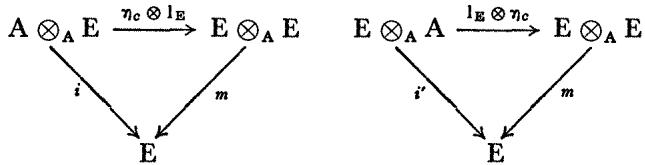
\includegraphics[keepaspectratio]{images/part003_ee0531f1.jpg}}

是交换的（其中 i 和 i' 表示典范同构（II，§3，第 4 号，命题 4））。

设 E 是一个具有单位元 e 的 A-代数，并设 \(\eta = \eta_{e}\) （也记作 \(\eta_{E}\) ）；则 \(\eta(\alpha\beta) = \eta(\alpha)\eta(\beta) = \alpha\eta(\beta)\) ，因为由（2）（第 1 号），

\[
(\alpha e) (\beta e) = (\alpha \beta) e = \alpha (\beta e);
\]

因此 \(\eta\) 是一个 A-代数同态。注意，E 上的 A-模结构可以利用 \(\eta\) 来定义，因为

\[
\alpha x = \eta (\alpha). x \quad \text { for } \alpha \in \mathrm{A}, x \in \mathrm{E}\tag{3}
\]

（其中右端的乘法在 E 中）。同态 \(\eta\) 的像是 E 的一个子代数，其元素与 E 的所有元素交换。同态 \(\eta\) 的核是 A-模 E 中元素 \(e\) 的零化子；由 (3)，它也是 A-模 E 的零化子（II，§ 1，第 12 号）。

当代数 E 含单位元且结合时， \(\eta\) 是一个环同态。反之，设 \(\rho:A\to B\) 是一个环同态，其像 \(\rho(A)\) 包含在 B 的中心内，并设环 A 交换；则在 B 上定义了一个结合且含单位元的 A-代数结构，其定义式为（参见 (3)）

\[
\lambda x = \rho (\lambda). x \quad \text { for } \lambda \in \mathbf {A}, x \in \mathbf {E}.
\]

\subsection{代数的乘积}

设 \((\mathbf{E}_i)_{i\in I}\) 是同一交换环 A 上的一族代数。立即可验证，在乘积集 \(\mathbf{E} = \prod_{i\in I}\mathbf{E}_i\) 上，乘积 A-模结构（II，§ 1，第 5 号）与乘法

\[
\left(\left(x _ {i}\right), \left(y _ {i}\right)\right) \mapsto \left(x _ {i} y _ {i}\right)\tag{4}
\]

定义了一个 A-代数结构；带此结构的集合 E 称为代数族 \((\mathbf{E}_{i})_{i\in I}\) 的积代数。

当所有代数 \(E_{t}\) 都为结合的（相应地，交换的，相应地，含单位元的）时，它们的积也是如此。此外，I，§ 8，第 10 号中所述的所有性质无需修改即可推广到代数的任意乘积。

\subsection{标量的限制与扩张}

设 \(A_{0}\) 和 A 是两个交换环，且 \(\rho:A_{0}\to A\) 是一个环同态。若 E 是一个 A-代数，我们（与 II，§ 1，第 13 号相一致地）用 \(\rho_{*}(E)\) 表示 \(A_{0}\) -模，它由 E 上的加法与外合成律

\[
\lambda . x = \rho (\lambda) x \quad \text { for   all } \lambda \in A _ {0} \text { and   all } x \in E.
\]

E 中的乘法与 \(A_{0}\) -模结构（在 \(\rho_{*}(E)\) 上）一起定义了一个 \(A_{0}\) -代数结构（在 \(\rho_{*}(E)\) 上）。当 \(A_{0}\) 是 A 的子环且 \(\rho\) 为典范单射时，称代数 \(\rho_{*}(E)\) 是由 E 把标量环 A 限制到 \(A_{0}\) 而得到的。作为语言上的滥用，当 \(\rho\) 任意时有时也这样说。

设 F 为一个 \(A_{0}\) -代数。 \(A_{0}\) -代数同态 \(F \to \rho_{*}(E)\) 称为半同态（相对于 \(\rho\) ），或 F 到 A-代数 E 中的 \(\rho\) -同态；若不致混淆，也称为 \(A_{0}\) -同态。若 E, \(E'\) 是两个 A-代数，则每个 A-代数同态 \(E \to E'\) 也是 \(A_{0}\) -代数同态 \(\rho_{*}(E) \to \rho_{*}(E')\) 。

现在考虑两个交换环 A 和 B 以及一个环同态 \(\rho: \mathbf{A} \to \mathbf{B}\) 。对每个 A-模 E，由 E 把标量环 A 扩张到 B 而得到的 B-模 \(\rho^{*}(\mathbf{E}) = \mathbf{E} \otimes_{\mathbf{A}} \mathbf{B}\) 已经定义（II，§ 5，第 1 号）。若 E 还是一个 A-代数，我们要在 \(\rho^{*}(\mathbf{E})\) 上定义一个 B-代数结构。为此，注意到 \((\mathbf{E} \otimes_{\mathbf{A}} \mathbf{B}) \otimes_{\mathbf{B}} (\mathbf{E} \otimes_{\mathbf{A}} \mathbf{B})\) 典范同构于 \((\mathbf{E} \otimes_{\mathbf{A}} \mathbf{E}) \otimes_{\mathbf{A}} \mathbf{B}\) （II，§ 5，第 1 号，命题 3）。若 \(m: \mathbf{E} \otimes_{\mathbf{A}} \mathbf{E} \to \mathbf{E}\) 定义 E 上的乘法，则映射 \(m \otimes l_{\mathbf{B}}: (\mathbf{E} \otimes_{\mathbf{A}} \mathbf{E}) \otimes_{\mathbf{A}} \mathbf{B} \to \mathbf{E} \otimes_{\mathbf{A}} \mathbf{B}\) 便典范地等同于一个 B-线性映射

\[
m ^ {\prime}: \rho^ {*} (\mathbf {E}) \otimes_ {\mathbf {B}} \rho^ {*} (\mathbf {E}) \rightarrow \rho^ {*} (\mathbf {E})
\]

它定义了 \(\rho^{*}(\mathbf{E})\) 上所要的 B-代数结构。于是

\[
(x \otimes \beta) (x ^ {\prime} \otimes \beta^ {\prime}) = (x x ^ {\prime}) \otimes (\beta \beta^ {\prime})\tag{5}
\]

对 \(x, x'\) （属于 \(\mathbf{E}\) ）与 \(\beta\) 、 \(\beta'\) （属于 \(\mathbf{B}\) ）成立，这便是所要的 B-代数结构。称 B-代数 \(\rho^*(\mathbf{E})\) 为由 A-代数 \(\mathbf{E}\) 通过把标量环 \(\mathbf{A}\) 扩张到 \(\mathbf{B}\) （借助 \(\rho\) ）而得到的代数。它也记作 \(\mathrm{E}_{(\mathbf{B})}\) 或 \(\mathbf{E} \otimes_{\mathbf{A}} \mathbf{B}\) 。当 \(\mathbf{E}\) 为结合的（相应地，交换的，相应地，含单位元的）时， \(\rho^*(\mathbf{E})\) 亦然。

对每个 A-代数 E，典范映射 \(\phi_{\mathbf{E}}: x \mapsto x \otimes 1\) （由 E 到 \(\mathrm{E}_{(\mathbf{B})}\) ）是一个代数的 A-同态。此外，对每个 B-代数 F 和每个 A-同态 \(f: \mathbf{E} \to \mathbf{F}\) ，存在唯一的 B-同态 \(\bar{f}: \mathbf{E}_{(\mathbf{B})} \to \mathbf{F}\) ，使得 \(\bar{f}(x \otimes 1) = f(x)\) 对所有 \(x \in \mathbf{E}\) 成立。

第一个断言由 \(\mathrm{E}_{(\mathrm{B})}\) 中乘法的定义直接得出，该定义给出 \((x\otimes1)(x'\otimes1)=(xx')\otimes1\) （对 \(x\in E\) 与 \(x'\in E\) ）。 B-线性映射 \(\bar{f}\) ——它由 \(\mathrm{E}_{(\mathrm{B})}\) 到 F 中、满足关系 \(\bar{f}(x\otimes1)=f(x)\) （对所有 \(x\in E\) ）——的存在性与唯一性由 II，§ 5，第 1 号，命题 1 得出；于是只需验证 \(\bar{f}(yy')=\bar{f}(y)\bar{f}(y')\) 对 y 与 \(y'\) （ \(\mathrm{E}_{(\mathrm{B})}\) 中的）成立；由于形如 \(x\otimes1\) （其中 \(x\in E\) ）的元素生成 B-模 \(\mathrm{E}_{(\mathrm{B})}\) ，只需考虑 \(y=x\otimes1\) , \(y'=x'\otimes1\) （其中 \(x\in E\) , \(x'\in E\) ）的情形；由于 \(yy'=(xx')\otimes1\) ，关系 \(\bar{f}(yy')=\bar{f}(y)\bar{f}(y')\) 便由 \(f(xx')=f(x)f(x')\) 得出。

也可以说 \(f \mapsto \bar{f}\) 是一个典范双射

\[
\operatorname{Hom} _ {\mathrm{A-alg.}} (\mathrm{E}, \rho_ {*} (\mathrm{F})) \rightarrow \operatorname{Hom} _ {\mathrm{B-alg.}} (\rho^ {*} (\mathrm{E}), \mathrm{F}).\tag{6}
\]

由 \(E_{(B)}\) 与 \(\phi_{E}\) 组成的有序对因此是泛映射问题（《集合论》，IV，§ 3，第 1 号）的一个解，其中 \(\Sigma\) 是 B-代数结构这个种类，而 \(\alpha\) -映射是 E 到 B-代数中的 A-同态。

推论。设 E, E' 为两个 A-代数；对代数的每个 A-同态 \(u: E \to E'\) ， \(u \otimes l_{B}\) 是使图表交换的唯一的代数 B-同态 v: \(E \otimes_{A} B \to E' \otimes_{A} B\)

\[
\begin{array}{c} \mathrm{E} \xrightarrow {\phi_ {\mathrm{E}}} \mathrm{E} \otimes_ {\mathrm{A}} \mathrm{B} \\ u \Biggl \downarrow \\ \mathrm{E} ^ {\prime} \xrightarrow [ \phi_ {\mathrm{E} ^ {\prime}} ]{} \mathrm{E} ^ {\prime} \otimes_ {\mathrm{A}} \mathrm{B} \end{array}
\]

设 C 为第三个交换环，且 \(\sigma: B \to C\) 为一个环同态；立即可见，典范 C-同态

\[
\sigma^ {*} (\rho^ {*} (\mathbf {E})) \rightarrow (\sigma \circ \rho) ^ {*} (\mathbf {E})
\]

把 \((x\otimes 1)\otimes 1\) 映为 \(x\otimes 1\) （对所有 \(x\in \mathbf{E}\) ）者（II，§ 5，第 1 号，命题 2）是一个代数同构。

\subsection{代数的逆向极限与正向极限}

设 I 是一个预序集， \((\mathbf{A}_{i},\phi_{ij})\) 是以 I 为指标集的交换环的逆向系统。设 \((\mathbf{E}_{i},f_{ij})\) 是以 I 为指标集的 \(A_{i}\) -模的逆向系统（II，§ 6，第 1 号），并进一步假设每个 \(E_{i}\) 具有 \(A_{i}\) -代数结构，且对 \(i\leqslant j,f_{ij}\) 是代数的 \(A_{j}\) -同态（相对于 \(\phi_{ij}\) ）（第 5 号）。设 \(A=\varprojlim A_{i}\) 与 \(E=\varprojlim E_{i}\) ，后者具有 A-模结构，即诸 \(\mathbf{A}_i\) -模 \(\mathbf{E}_i\) 的结构的逆向极限（II，§ 6，第 1 号）；立即可验证， \(\mathbf{E}\) 上的合成律——把诸 \(\mathbf{E}_i\) 视为乘法下的广群（I，§ 10，第 1 号）而取其逆向极限——连同 \(\mathbf{E}\) 上的 A-模结构，在 \(\mathbf{E}\) 上定义了一个 A-代数结构； \((\mathbf{E}_i, f_{ij})\) 称为 \(\mathbf{A}_i\) -代数的逆向系统，而 A-代数 \(\mathbf{E}\) 称为其逆向极限。若 \(f_i: \mathbf{E} \to \mathbf{E}_i\) , \(\phi_i: \mathbf{A} \to \mathbf{A}_i\) 为典范映射，则 \(f_i\) 是代数的 A-同态（相对于 \(\phi_i\) ）。若诸 \(\mathbf{E}_i\) 结合（相应地，交换），则 \(\mathbf{E}\) 亦然；若每个 \(\mathbf{E}_i\) 具有单位元 \(e_i\) 且 \(f_{ij}(e_j) = e_i\) （对 \(i \leqslant j\) ），则 \(e = (e_i)\) 是代数 \(\mathbf{E}\) 的单位元。

设 \((\mathbf{E}_{i}^{\prime}, f_{ij}^{\prime})\) 是 \(A_{i}\) -代数的另一个逆向系统，且对所有 i 令 \(u_{i}: E_{i} \to E_{i}^{\prime}\) 为 \(A_{i}\) -代数同态，这些映射构成一个逆向系统；则 \(u = \lim u_{i}\) 是一个 A-代数同态。

现在假设所有的 \(A_{i}\) 都等于同一个交换环 A，且诸 \(\phi_{ij}\) 等于 \(Id_{A}\) ，于是 \(E = \lim E_{i}\) 是一个 A-代数。设 F 是一个 A-代数，且对所有 \(i \in I\) ，设 \(u_{i}: F \to E_{i}\) 是一个 A-代数同态，使得 \((u_{i})\) 是一个映射的逆向系统；则 \(u = \lim u_{i}\) 是代数 F 到代数 E 中的同态。反之，对每个 A-代数同态 \(v: F \to E\) ，族 \(v_{i} = f_{i} \circ v\) 是一个 A-代数同态的逆向系统，使得 \(v = \lim v_{i}\) 。此外，由于记 \(\bar{f}_{ij} = \text{Hom}(1_{\text{F}}, f_{ij})\) , \((\text{Hom}_{\text{A-alg.}}(\text{F}, \text{E}_i), \bar{f}_{ij})\) 显然是一个集合的逆向系统，可见上述评注也可以表述为：典范映射 \(v \mapsto (f_i \circ v)\) 是一个双射

\[
l _ {\mathrm{F}}: \operatorname{Hom} _ {\mathrm{A-alg.}} (\mathrm{F}, \varprojlim \mathrm{E} _ {i}) \rightarrow \varprojlim \operatorname{Hom} _ {\mathrm{A-alg.}} (\mathrm{F}, \mathrm{E} _ {i}).
\]

此外，对于每一个 A-代数同态 \(w: \mathbf{F} \to \mathbf{F}'\) ，

\[
\bar {w} _ {i} = \operatorname{Hom} (w, 1 _ {\mathrm{E} _ {i}}): \operatorname{Hom} _ {\mathrm{A-alg.}} (\mathrm{F} ^ {\prime}, \mathrm{E} _ {i}) \rightarrow \operatorname{Hom} _ {\mathrm{A-alg.}} (\mathrm{F}, \mathrm{E} _ {i})
\]

构成映射的逆向系统，且图表

\[
\begin{array}{c} \operatorname{Hom} _ {\mathrm{A-alg.}} (\mathrm{F} ^ {\prime}, \lim \mathrm{E} _ {i}) \xrightarrow {l _ {\mathbf {F} ^ {\prime}}} \lim \operatorname{Hom} _ {\mathrm{A-alg.}} (\mathrm{F} ^ {\prime}, \mathrm{E} _ {i}) \\ \operatorname{Hom} (w, 1 _ {\mathbf {E}}) \Biggl \downarrow \qquad \qquad \qquad \qquad \qquad \qquad \qquad \qquad \qquad \qquad \qquad \qquad \qquad \qquad \qquad \qquad \qquad \qquad \qquad \qquad \qquad \qquad \qquad \qquad \qquad \qquad \qquad \qquad \qquad \qquad \qquad \qquad \qquad \qquad \\ \operatorname{Hom} _ {\mathrm{A-alg.}} (\mathrm{F}, \lim \mathrm{E} _ {i}) \xrightarrow {l _ {\mathbf {F}}} \lim \operatorname{Hom} _ {\mathrm{A-alg.}} (\mathrm{F}, \mathrm{E} _ {i}) \end{array}
\]

是交换的。

现在假设 I 是右有向的。考虑交换环的正向系统 \((\mathbf{A}_i, \phi_{ji})\) 与正向系统 \((\mathbf{E}_i, f_{ji})\) （ \(\mathbf{A}_i\) -模的），均以 I 为指标集；假设每个 \(\mathbf{E}_i\) 具有 \(\mathbf{A}_i\) -代数结构，且对 \(i \leqslant j\) ， \(f_{ji}\) 是代数的 \(\mathbf{A}_i\) -同态（相对于 \(\phi_{ji}\) ）（第 5 号）。设 \(\mathbf{A} = \varinjlim \mathbf{A}_i\) , \(\mathbf{E} = \varinjlim \mathbf{E}_i\) ； \(\mathbf{E}\) 具有 A-模结构，即诸 \(\mathbf{A}_i\) -模 \(\mathbf{E}_i\) 的结构的正向极限（II，§ 6，第 2 号）；此外，E 上的合成律——把诸 \(E_{i}\) 视为乘法下的广群（I，§ 10，第 3 号）而取其正向极限——连同 E 上的 A-模结构，在 E 上定义了一个 A-代数结构； \((\mathbf{E}_{i}, f_{jt})\) 称为 \(A_{i}\) -代数的正向系统，而 A-代数 E 称为其正向极限。若 \(f_{i}: E_{i} \to E\) , \(\phi_{i}: A_{i} \to A\) 为典范映射，则 \(f_{i}\) 是代数的 \(A_{i}\) -同态（相对于 \(\phi_{i}\) ）。若诸 \(E_{i}\) 结合（相应地，交换），则 E 亦然；若每个 \(E_{i}\) 具有单位元 \(e_{i}\) 且 \(f_{jt}(e_{i}) = e_{j}\) （对 \(i \leqslant j\) ），则 E 具有单位元 e，使得 \(f_{i}(e_{i}) = e\) 对所有 \(i \in I\) 成立。

设 \((\mathbf{E}_i', f_{ji}')\) 是 \(\mathbf{A}_i\) -代数的另一个正向系统，且对所有 \(i\) ，设 \(u_i: \mathbf{E}_i \to \mathbf{E}_i'\) 为 \(\mathbf{A}_i\) -代数同态，这些映射构成一个正向系统；则 \(u = \lim u_i\) 是一个 \(\mathbf{A}\) -代数同态。

现在假设所有的环 \(\mathbf{A}_i\) 都等于同一个环 \(\mathbf{A}\) ，且诸 \(\phi_{ji}\) 等于 \(\mathrm{Id}_{\mathbf{A}}\) ，于是 \(\mathbf{E} = \varinjlim \mathbf{E}_i\) 是一个 A-代数。设 \(\mathbf{F}\) 是一个 A-代数，且对所有 \(i\) ，设 \(u_i: \mathbf{E}_i \to \mathbf{F}\) 是一个 A-代数同态，使得 \((u_i)\) 是一个映射的正向系统；则 \(u = \varinjlim u_i\) 是代数 \(\mathbf{E}\) 到代数 \(\mathbf{F}\) 中的同态。反之，对每个 A-代数同态 \(v: \mathbf{E} \to \mathbf{F}\) ，族 \(v_i = v \circ f_i\) 是一个 A-代数同态的正向系统，使得 \(v = \varinjlim v_i\) 。此外，由于记 \(\bar{f}_{ij} = \operatorname{Hom}(f_{ij}, 1_F)\) , \((\operatorname{Hom}_{\mathbf{A-alg}}(\mathbf{E}_i, \mathbf{F}), \bar{f}_{ij})\) 显然是一个集合的逆向系统，可见上述评注也可以表述为：典范映射 \(v \mapsto (v \circ f_i)\) 是一个双射

\[
d _ {\mathrm{F}}: \operatorname{Hom} _ {\mathrm{A-alg.}} (\varinjlim \mathrm{E} _ {i}, \mathrm{F}) \rightarrow \varprojlim \operatorname{Hom} _ {\mathrm{A-alg.}} (\mathrm{E} _ {i}, \mathrm{F}).
\]

进一步地，对于每个A-代数同态 \(w: F \rightarrow F'\) ，

\[
\bar {w} _ {i} = \operatorname{Hom} (1 _ {\mathrm{E} _ {i}}, w): \operatorname{Hom} _ {\mathrm{A-alg.}} (\mathrm{E} _ {i}, \mathrm{F}) \rightarrow \operatorname{Hom} _ {\mathrm{A-alg.}} (\mathrm{E} _ {i}, \mathrm{F} ^ {\prime})
\]

构成映射的逆向系统，且图表

\[
\begin{array}{l} \operatorname{Hom} _ {\mathrm{A-alg.}} (\varinjlim \mathrm{E} _ {i}, \mathrm{F}) \xrightarrow {d _ {\mathrm{F}}} \varprojlim \operatorname{Hom} _ {\mathrm{A-alg.}} (\mathrm{E} _ {i}, \mathrm{F}) \\ \operatorname{Hom} (1 _ {\mathrm{E}}, w) \Biggl \downarrow \qquad \qquad \qquad \qquad \qquad \qquad \qquad \qquad \qquad \qquad \qquad \qquad \qquad \qquad \qquad \qquad \qquad \qquad \qquad \qquad \varprojlim \varpi_ {i} \\ \operatorname{Hom} _ {\mathrm{A-alg.}} (\varinjlim \mathrm{E} _ {i}, \mathrm{F} ^ {\prime}) \xrightarrow {d _ {\mathrm{F} ^ {\prime}}} \varprojlim \operatorname{Hom} _ {\mathrm{A-alg.}} (\mathrm{E} _ {i}, \mathrm{F} ^ {\prime}) \end{array}
\]

是交换的。

\subsection{代数的基。乘法表}

根据定义，A-代数 E 的基就是 E 的 A-模结构的基。设 \((a_{i})_{i\in I}\) 是 E 的一组基；存在唯一的由环 A 的元素组成的族 \((\gamma_{ij}^{k})_{(i,j,k)\in I\times I\times I}\) ，使得对每个有序对 \((i,j)\in I\times I\) ， \(k\in I\) 中使 \(\gamma_{ij}^{k}\neq 0\) 者只有有限多个，且

\[
a _ {i} a _ {j} = \sum_ {k \in \mathbf {I}} \gamma_ {i j} ^ {k} a _ {k}.\tag{7}
\]

诸 \(\gamma_{ij}^{k}\) 称为代数 E 关于基 \((a_{i})\) 的结构常数，而关系式 (7) 构成代数 E （相对于基 \((a_{i})\) ）的乘法表。

关系式（7）可以想象为将这些关系式的右端排列在一个方形表格中写出。

\(\cdots\)

\(a_j\)

\(\cdots\)

\(\vdots\)

\(a_j\)

\(\sum_{k} \gamma_{ij}^{k} a_k\)

\(\vdots\)

这里约定，第 i 行第 j 列处的元素等于乘积 \(a_{i}a_{j}\) 。

反之，给定一个 A-模 E、E 的基 \((a_{i})_{i\in I}\) 以及 A 的元素的一个族 \((\gamma_{ij}^{k})\) ，使得对每个有序对 \((i,j)\in I\times I\) ， \(k\in I\) 中使 \(\gamma_{ij}^{k}\neq 0\) 者只有有限多个，则在 E 上存在唯一的 A-代数结构使关系式 (7) 成立，因为 A-模 \(\mathbf{E}\otimes_{\mathbf{A}}\mathbf{E}\) 是自由的，且以 \((a_{i}\otimes a_{j})_{(i,j)\in I\times I}\) 为基（参见 II，§ 3，第 7 号，命题 7 的推论 2）。

设 E 是一个 A-代数， \((a_{i})_{i\in I}\) 是 A-模 E 的一个生成系（例如一组基）。要使 E 为结合的，必要且充分的条件是诸 \(a_{i}\) 满足结合性关系

\[
(a _ {i} a _ {j}) a _ {k} = a _ {i} (a _ {j} a _ {k}) \quad \text { for   all } i, j, k\tag{8}
\]

映射 \((x, y, z) \mapsto (xy)z - x(yz)\) 是一个 A-三线性映射

\[
\mathbf {E} \times \mathbf {E} \times \mathbf {E} \rightarrow \mathbf {E}
\]

从而定义了一个 A-线性映射 \(E \otimes_{A} E \otimes_{A} E \to E\) ；若后一映射对所有元素 \(a_{i} \otimes a_{j} \otimes a_{k}\) （它们构成 A-模 \(E \otimes_{A} E \otimes_{A} E\) 的一个生成系）均为零，则它恒为零。

类似地，要使 E 为交换的，必要且充分的条件是诸 \(a_{i}\) 满足交换性关系

\[
a _ {i} a _ {j} = a _ {j} a _ {i} \quad \text { for   all } i, j.\tag{9}
\]

证明是类似的，这次考虑 A-双线性映射 \((x,y)\mapsto xy - yx\) 。最后，要使元素 \(e\in E\) 成为单位元，必要且充分的条件是诸 \(a_{i}\) 满足关系

\[
a _ {i} = e a _ {i} = a _ {i} e \quad \text { for   all } i,\tag{10}
\]

这一次是借助 A-线性映射 \(x \mapsto x - xe\) 与 \(x \mapsto x - ex\) 看出的。

当 \((a_{i})_{i\in I}\) 是 E 的一组基且 \((\gamma_{ij}^{k})\) 是相应的结构常数族时，关系式 (8) 等价于关系式

\[
\sum_ {r} \gamma_ {i j} ^ {r} \gamma_ {r k} ^ {s} = \sum_ {r} \gamma_ {i r} ^ {s} \gamma_ {j k} ^ {r}
\]

对所有 \(i, j, k, s\) 成立。类似地，关系式 (9) 等价于 \(\gamma_{ij}^{k} = \gamma_{ji}^{k}\) （对所有 \(i, j, k\) ）。

设 \((a_{i})_{i\in I}\) 是 A-代数 E 的一组基；若 \(\rho :A\to B\) 是一个环同态，则 \((a_{i}\otimes 1)\) 是 B-代数 \(\rho^{*}(\mathbf{E}) = \mathbf{E}\otimes_{\mathbf{A}}\mathbf{B}\) 的一组基（II，§ 5，第 1 号，命题 4）。若 \((\gamma_{ij}^{k})\) 是关于基 \((a_{i})\) 的结构常数族，则族 \((\rho (\gamma_{ij}^{k}))\) 是 \(\rho^{*}(\mathbf{E})\) 关于基 \((a_{i}\otimes 1)\) 的结构常数族。

\section{代数的例子}

在本段中，A 表示一个交换环。

\subsection{自同态代数}

设 B 是一个带单位元（记为 1）的结合 A-代数，并设 M 是一个右 B-模。我们知道环 \(\mathbf{E} = \operatorname{End}_{\mathbf{B}}(\mathbf{M})\) 在 B 的中心上也具有一个模结构。现在，由 A 到 B 的同态 \(h: \alpha \mapsto \alpha\) . 1 的像包含在 B 的中心中（ \(\S 1\) ，第 1 号）；因此 \(h\) 给 E 一个 A-模结构。此外，对 \(\alpha \in \mathbf{A}\) 与 E 中的 \(f, g\) ，

\[
\alpha (f \circ g) = f \circ (\alpha g) = (\alpha f) \circ g;
\]

因此 E 中的乘法与 E 上的 A-模结构定义了 E 上的一个结合 A-代数结构；M 的恒等映射是该代数的一个单位元。

\subsection{矩阵元素}

设 B 为含单位元的结合 A-代数， \(\mathbf{M}_{n}(\mathrm{B})\) 为 B 上 n 阶方阵的集合（II，§ 10，第 7 号）。则 \(\mathbf{M}_{n}(\mathrm{B})\) 具有 A-模结构，定义为 \(\alpha.(b_{ij})=(\alpha b_{ij})(\alpha\in\mathrm{A},b_{ij}\in\mathrm{B},1\leqslant i\leqslant n,1\leqslant j\leqslant n)\) ；此结构与矩阵乘法在 \(\mathbf{M}_{n}(\mathrm{B})\) 上定义了一个含单位元的结合 A-代数结构。 \(\mathbf{M}_{n}(\mathrm{B})\) 到 \(\operatorname{End}_{\mathrm{B}}(\mathrm{B}_{d}^{n})\) 上的典范双射（II，§ 10，第 7 号）是一个 A-代数同构。

当 B = A 时，A-代数 \(\mathbf{M}_{n}(\mathbf{A})\) 具有由矩阵单位（II，§ 10，第 3 号）组成的典范基 \((E_{ij})\) ；相应的乘法表为

\[
E _ {i j} E _ {h k} = \delta_ {j h} \mathrm{E} _ {i k}.\tag{1}
\]

单位元 \(I_{n}\) 等于 \(\sum_{i=1}^{n} E_{ii}\) 。

\subsection{二次代数}

设 \(\alpha, \beta\) 是 A 的两个元素， \((e_1, e_2)\) 是 \(\mathbf{A}^2\) 的典范基。A 上 \((\alpha, \beta)\) 型的二次代数是指带有由乘法表（§ 1，第 7 号）定义的代数结构的 A-模 \(\mathbf{A}^2\)

\[
e _ {1} ^ {2} = e _ {1}, \qquad e _ {1} e _ {2} = e _ {2} e _ {1} = e _ {2}, \qquad e _ {2} ^ {2} = \alpha e _ {1} + \beta e _ {2}.\tag{2}
\]

一个与二次代数同构的A-代数E也称为二次代数。这等同于说E有一个由两个元素组成的基，其中一个为单位元。

可以证明，每个具有由两个元素组成的基的含单位元 A-代数都是二次代数（习题 1）。

若 A-代数的一个基 \((e_{1}, e_{2})\) 的乘法表为 (2)，则称它为 \((\alpha, \beta)\) 型的基。作为语言上的滥用，当一个二次代数具有 \((\alpha, \beta)\) 型的基时，就说它是 \((\alpha, \beta)\) 型的。

命题 1. 二次代数 E 是结合的且交换的。

E 的交换性由 (2) 中的关系式 \(e_{1}e_{2}=e_{2}e_{1}\) 得出；类似地，要验证结合性，只需验证 \(x(yz)=(xy)z\) 当 x, y, z 各取 \(e_{1}\) 或 \(e_{2}\) 时成立。现在，若 x, y, z 中至少有一个等于 \(e_{1}\) ，则此关系显然成立；对 x=y=z=e₂ 也成立，因为 E 交换；命题得证。

设 \(e\) 表示二次代数 \(\mathbf{E}\) 的单位元， \((e, i)\) 是 \(\mathbf{E}\) 的 \((\alpha, \beta)\) 型基； \(\mathbf{E}\) 的包含 \(e\) 的任何其他基因此形如 \((e, j)\) ，其中 \(j = \gamma e + \delta i\) （II，§ 7，第 2 号，命题 3 的推论）；此外， \((e, j)\) 为 \(\mathbf{E}\) 的基的必要且充分条件是 \(\delta\) 在 \(\mathbf{A}\) 中可逆；该条件显然充分；反之，若 \(i\) 是 \(i\) 在 \(\mathbf{E}/\mathbf{A}e\) 中的典范像，则 \(i\) 与 \(\bar{j} = \delta i\) 都必须构成 \(\mathbf{E}/\mathbf{A}e\) 的基，由此得该条件的必要性。于是

\[
j ^ {2} = (\gamma^ {2} + \alpha \delta^ {2}) e + (2 \gamma \delta + \beta \delta^ {2}) i = (\alpha \delta^ {2} - \gamma^ {2} - \beta \gamma \delta) e + (2 \gamma + \beta \delta) j;
\]

由此看出 E 是以下类型的

\[
(\alpha \delta^ {2} - \gamma^ {2} - \beta \gamma \delta , 2 \gamma + \beta \delta)\tag{3}
\]

对所有可逆的 \(\delta \in \mathbf{A}\) 以及所有 \(\gamma \in \mathbf{A}\) 。特别地，若 \(\mathbf{E}\) 是 \((\alpha, 2\beta')\) 型的，则 E 也是 \((\alpha + \beta'^2, 0)\) 型的，这可由取 \(\gamma = -\beta'\) 与 \(\delta = 1\) 看出。

命题 2. 设 E 是一个二次 A-代数，e 是它的单位元。对所有 \(u \in \mathbf{E}\) ，设 \(\mathrm{T}(u)\) 是自由 A-模 E 的自同态 \(m_u: x \mapsto ux\) 的迹（II，§ 4，第 3 号）。则映射 \(s\) ——定义为 \(s(u) = \mathrm{T}(u)\) . \(e - u\) ——是代数 E 的一个自同构，且 \(s^2(u) = u\) 对所有 \(u \in \mathbf{E}\) 成立。

设 \((e, i)\) 是 E 的 \((\alpha, \beta)\) 型基；则 \(T(e) = 2\) ，从而 \(s(e) = e\) ，且 \(T(i) = \beta\) ，从而 \(s(i) = \beta e - i\) 。于是 \((e, s(i))\) 是 E 的基，其类型由 (3) 给出，其中 \(\gamma = \beta\) 且 \(\delta = -1\) ，这重新给出 \((\alpha, \beta)\) ；由此得出 \(s\) 是代数 E 的自同构。由于 \(m_{s(u)} = sm_u s^{-1}\) ，A-模 E 的自同态 \(m_u\) 与 \(m_{s(u)}\) 具有相同的迹（II，§ 4，第 3 号，命题 3），因此

\[
s ^ {2} (u) = \mathrm{T} (u). e - s (u) = \mathrm{T} (u). e - (\mathrm{T} (u). e - u) = u
\]

对所有 \(u \in E\) 成立。

自同构 \(s\) 称为 A-代数 \(\mathbf{E}\) 的共轭，而 \(s(u)\) 称为 \(u\) 的共轭元。

若 \(u = \xi e + \eta i\) ，其中 \(\xi, \eta\) 属于 \(A\) ，则 \(s(u) = (\xi + \beta \eta)e - \eta i\) ，从而

\begin{enumerate}
\def\labelenumi{(\arabic{enumi})}
\setcounter{enumi}{3}
\tightlist
\item
\end{enumerate}

\[
\mathrm{T} (u) e = u + s (u) = (2 \xi + \beta \eta) e\tag{5}
\]

\[
u. s (u) = (\xi^ {2} + \beta \xi \eta - \alpha \eta^ {2}) e = N (u) e
\]

其中我们记 \(\mathrm{N}(u)=\xi^{2}+\beta\xi\eta-\alpha\eta^{2}\) 。元素 \(\mathrm{T}(u)\) 与 \(\mathrm{N}(u)\) （或当 A 与 Ae 典范地等同时的元素 \(\mathrm{T}(u)e\) 与 \(\mathrm{N}(u)e\) ）分别称为 u 的迹与范数。

当 \(\beta = 0\) 时，上述公式简化为

\[
s (\xi e + \eta i) = \xi e - \eta i, \quad \mathrm{T} (\xi e + \eta i) = 2 \xi , \quad \mathrm{N} (\xi e + \eta i) = \xi^ {2} - \alpha \eta^ {2}. \tag {6}
\]

显然，T 是 E 上的线性形式，N 是 E 上的二次形式（IX，§ 3，第 4 号）。由于 E 交换且结合，由 (5) 可得

\[
\mathrm{N} (u v) = \mathrm{N} (u)) \mathrm{N} (v).\tag{7}
\]

要使 u 在 E 中可逆，必要且充分的条件是 \(\mathrm{N}(u)\) 在 A 中可逆。因为由 \(\mathrm{N}(e)=1\) ，取 \(v=u^{-1}\) 便由 (7) 得出条件的必要性。反之，若 \(\mathrm{N}(u)\) 在 A 中可逆，则由 (5) 知 u 可逆，且

\[
u ^ {- 1} = (\mathrm{N} (u)) ^ {- 1} s (u).\tag{8}
\]

可以证明 \(\mathbf{N}(u)\) 是自同态 \(m_u\) 的行列式（§ 8，第 1 号）（参见 § 9 第 3 号，例 1）。

如下命题给出了交换域上二次代数的结构：

命题 3. 设 E 是一个 \((\alpha, \beta)\) 型的二次 A-代数。

\begin{enumerate}
\def\labelenumi{(\roman{enumi})}
\item
  若 \(\mathbf{A}\) 是一个域，且不包含任何元素 \(\zeta\) 使得 \(\zeta^2 = \alpha + \beta \zeta\) ，则 \(\mathbf{E}\) 是 \(a\) （交换）域（参见 V，§ 3）。
\item
  若环 A 含有元素 \(\zeta\) 使得 \(\zeta^2 = \alpha + \beta\zeta\) ，且 \(\beta - 2\zeta\) 可逆（相应地，为零），则 E 同构于 \(\mathbf{A} \times \mathbf{A}\) （相应地，是 \((0,0)\) 型的）。
\end{enumerate}

我们证明 (i)。设 \(\xi, \eta\) 是 A 的两个元素，且 \(u = \xi e + \eta i\) 。若 \(\eta \neq 0\) ，写 \(\theta = -\xi \eta^{-1}\) ，则由 (5) 得 \(\mathrm{N}(u) = \eta^2 (\theta^2 - \beta \theta - \alpha)\) ，于是由对 A 的假设得 \(\mathrm{N}(u) \neq 0\) ；若 \(\eta = 0\) ，则 \(\mathrm{N}(u) = \xi^2\) 。无论哪种情形，若 \(u \neq 0\) ，则 \(\mathrm{N}(u) \neq 0\) ，从而 \(\mathrm{N}(u)\) 在 A 中可逆，因而 \(u\) 在 E 中可逆。

我们现在证明 (ii)。典范基 \((e_{1}, e_{2})\) （代数 \(A \times A\) 的）是 \((0, 1)\) 型的。我们已见（公式 (3)）E 的类型为

\[
(\alpha \delta^ {2} - \gamma^ {2} - \beta \gamma \delta , 2 \gamma + \beta \delta)
\]

对所有 \(\gamma \in \mathbf{A}\) 以及所有 \(\delta\) （在 \(\mathbf{A}\) 中可逆的）。若 \(\beta - 2\zeta\) 可逆，取 \(\delta = (\beta - 2\zeta)^{-1}\) 与 \(\gamma = -\zeta(\beta - 2\zeta)^{-1}\) ；则 \(2\gamma + \beta\delta = 1\) ，且

\[
\alpha \delta^ {2} - \gamma^ {2} - \beta \gamma \delta = \delta^ {2} (\alpha - \zeta^ {2} + \beta \zeta) = 0;
\]

于是 E 是 \((0,1)\) 型的，从而同构于 A × A。若 \(\beta - 2\zeta = 0\) ，则已指出 E 是 \((\alpha + \zeta^{2}, 0)\) 型的，从而是 \((0,0)\) 型的，因为 \(\alpha + \zeta^{2} = 2\zeta^{2} - \beta\zeta = 0\) 。

\((0,0)\) 型的二次 A-代数也称为 A 上的对偶数代数。

\subsection{凯莱代数}

定义 1. \(\mathbf{A}\) 上的一个凯莱代数是指一个有序对 \((\mathbf{E}, s)\) ，其中 \(\mathbf{E}\) 是 \(\mathbf{A}\) 上的一个带单位元 \(e\) 的代数，而 \(s\) 是 \(\mathbf{E}\) 的一个反自同构，使得

\[
u + s (u) \in \mathrm{A} e \quad \text { and } \quad u. s (u) \in \mathrm{A} e
\]

对所有 \(u \in \mathbf{E}\) 成立。

s 称为凯莱代数 (E, s) 的共轭，而 \(s(u)\) 称为 u 的共轭元。条件 \(u + s(u) \in Ae\) 蕴含 u 与 \(s(u)\) 可交换。我们记

\begin{enumerate}
\def\labelenumi{(\arabic{enumi})}
\setcounter{enumi}{8}
\tightlist
\item
\end{enumerate}

\[
\mathrm{T} (u) = u + s (u)\tag{10}
\]

\[
\mathrm{N} (u) = u. s (u) = s (u). u
\]

而子代数 Ae 的这些元素分别称为 u 的凯莱迹与范数。

由二次代数 E 及其共轭 s（因 E 交换，故 s 是反自同构）（第 3 号）组成的有序对是一个凯莱代数。

设 \((\mathbf{E}, s)\) 是一个凯莱代数；由于 \(s(e) = e\) ，有 \(s(u + s(u)) = u + s(u)\) ，换言之 \(s(u) + s^2(u) = u + s(u)\) ，或等价地

\[
s ^ {2} (u) = u\tag{11}
\]

于是 \(s^{2}\) 是 E 的恒等映射。由此可得

\[
\mathrm{T} (s (u)) = \mathrm{T} (u), \quad \mathrm{N} (s (u)) = \mathrm{N} (u).\tag{12}
\]

最后，关系式 \((u - u)(u - s(u)) = 0\) 给出

\[
u ^ {2} - \mathrm{T} (u). u + \mathrm{N} (u) = 0\tag{13}
\]

对所有 \(u \in \mathbf{E}\) 成立。

命题 4. 设 E 是一个 A-代数，s 与 \(s'\) 是 E 的反自同构，使得 \((E, s)\) 与 \((E, s')\) 是凯莱代数。若 E 有一个包含单位元 e 的基，则 \(s' = s\) 。

显然 \(s'(u) = s(u) = u\) 对所有 \(u \in Ae\) 成立。若 T, N（相应地，T', N'）是 (E, s)（相应地，(E, s')）的迹函数与范数函数，则由 (13) 可得

\[
(\mathrm{T} (u) - \mathrm{T} ^ {\prime} (u)). u - (\mathrm{N} (u) - \mathrm{N} ^ {\prime} (u)) = 0.
\]

设 B 是 E 的一个包含 e 的基，u 是 B 中异于 e 的一个元素；则 \(\mathrm{T}(u) - \mathrm{T}'(u) = 0\) ，从而 \(s(u) = s'(u)\) 。由于 s 与 \(s'\) 在 B 上重合，故二者相等。

在下文中我们将记 \(\bar{u} = s(u)\) ，于是

\[
\left\{ \begin{array}{l l} u + \bar {u} = \mathrm{T} (u), & u \bar {u} = \bar {u} u = \mathrm{N} (u), \quad \bar {\bar {u}} = u \\ \overline {{u + v}} = \bar {u} + \bar {v}, & \overline {{\alpha u}} = \alpha \bar {u}, \quad \overline {{u v}} = \bar {v}. \bar {u} \end{array} \right.\tag{14}
\]

其中 \(u, v\) 属于 \(\mathbf{E}, \alpha \in \mathbf{A}\) ；此外

\[
\mathbf {T} (e) = 2 e, \quad \mathbf {N} (e) = e.\tag{15}
\]

由公式

\[
\mathrm{T} (u v) = u v + \overline {{{{u v}}}} = u v + \bar {v}. \bar {u} = u v + (\mathrm{T} (v) - v) (\mathrm{T} (u) - u),
\]

我们推出

\[
u v + v u = \mathrm{T} (u) v + \mathrm{T} (v) u + (\mathrm{T} (u v) - \mathrm{T} (u) \mathrm{T} (v))\tag{16}
\]

由此，交换 \(u\) 与 \(v\) ，得

\[
\mathbf {T} (v u) = \mathbf {T} (u v).\tag{17}
\]

另一方面， \(\mathrm{N}(u+v)=(u+v)(\bar{u}+\bar{v})=\mathrm{N}(u)+\mathrm{N}(v)+\mathrm{T}(u\bar{v})\) ，从而

\[
\mathrm{T} (v \bar {u}) = \mathrm{T} (u \bar {v}) = \mathrm{N} (u + v) - \mathrm{N} (u) - \mathrm{N} (v).\tag{18}
\]

现在，把 (16) 中的 u 换成 \(\bar{u}\) 便得到

\[
\mathrm{T} (u \bar {v}) = \mathrm{T} (u) \mathrm{T} (v) + \bar {u} v + v \bar {u} - \mathrm{T} (u) v - \mathrm{T} (v) \bar {u} = \mathrm{T} (u) \mathrm{T} (v) - u v - \bar {v}. \bar {u};
\]

从而

\[
\mathrm{T} (v \bar {u}) = \mathrm{T} (u \bar {v}) = \mathrm{N} (u + v) - \mathrm{N} (u) - \mathrm{N} (v) = \mathrm{T} (u) \mathrm{T} (v) - \mathrm{T} (u v).\tag{19}
\]

最后，显然对所有 \(\alpha \in \mathbf{A}\) ，

\[
\mathrm{N} (\alpha u) = \alpha^ {2} \mathrm{N} (u);\tag{20}
\]

特别地 \(\mathbf{N}(2u) = 4\mathbf{N}(u)\) ，于是公式 (19) 给出

\[
(\mathrm{T} (u)) ^ {2} - \mathrm{T} (u ^ {2}) = 2 \mathrm{N} (u).\tag{21}
\]

显然 T 是 (Ae)-模 E 上的线性形式。由于 \((u, v) \mapsto \mathrm{T}(v\bar{u})\) 是该模上的双线性形式，由 (18) 与 (20) 可知 N 是一个二次型（参见 IX，§ 3，第 4 号）。

\subsection{凯莱代数的构造。四元数}

设 \((\mathbf{E}, s)\) 是 A 上的一个凯莱代数（对它我们将使用第 4 号的记号），并设 \(\gamma \in \mathbf{A}\) 。设 F 是 A 上的这样的代数：其底模为 \(\mathbf{E} \times \mathbf{E}\) ，乘法由下式定义

\[
(x, y) (x ^ {\prime}, y ^ {\prime}) = (x x ^ {\prime} + \gamma \bar {y} ^ {\prime} y, y \bar {x} ^ {\prime} + y ^ {\prime} x);\tag{22}
\]

显然 \((e,0)\) 是 F 的单位元，且 \(E \times \{0\}\) 是 F 的一个与 E 同构的子代数；在下文中我们把它与 E 等同，于是 \(x \in E\) 与 \((x,0)\) 等同，特别地，e 与 F 的单位元等同。

设 \(t\) 是 \(\mathbf{F}\) 的由下式定义的置换

\begin{enumerate}
\def\labelenumi{(\arabic{enumi})}
\setcounter{enumi}{22}
\tightlist
\item
\end{enumerate}

\[
t ((x, y)) = (\bar {x}, - y) \quad (x \in \mathbf {E}, y \in \mathbf {E}).
\]

命题 5. (i) 有序对 \((\mathbf{F}, t)\) 是 \(\mathbf{A}\) 上的一个凯莱代数。

\begin{enumerate}
\def\labelenumi{(\roman{enumi})}
\setcounter{enumi}{1}
\tightlist
\item
  设 \(j = (0, e)\) ，从而 \((x, y) = xe + yj\) （对 \(x \in \mathbf{E}\) ， \(y \in \mathbf{E}\) ）。 \(\mathbf{T}_{\mathbb{F}}\) 与 \(\mathbf{N}_{\mathbb{F}}\) （ \(\mathbf{F}\) 的凯莱迹与范数）由下列公式给出
\end{enumerate}

\[
\mathrm{T} _ {\mathrm{F}} (x e + y j) = \mathrm{T} (x), \quad \mathrm{N} _ {\mathrm{F}} (x e + y j) = \mathrm{N} (x) - \gamma \mathrm{N} (y).\tag{24}
\]

\begin{enumerate}
\def\labelenumi{(\roman{enumi})}
\setcounter{enumi}{2}
\tightlist
\item
  要使 F 为结合的，必要且充分的条件是 E 为结合的且交换的。
\end{enumerate}

对 \((x,y)\in \mathbf{F},\)

\begin{enumerate}
\def\labelenumi{(\arabic{enumi})}
\setcounter{enumi}{24}
\tightlist
\item
\end{enumerate}

\[
\begin{array}{r l r} & & {(x, y) + t ((x, y)) = (x + \bar {x}, 0) = \mathrm{T} (x) e} \\ & & {(x, y) t ((x, y)) = (x, y) (\bar {x}, - y) = (x \bar {x} - \gamma \bar {y} y, y \bar {\bar {x}} - y x)} \\ & & {= (\mathrm{N} (x) - \gamma \mathrm{N} (y), 0) = (\mathrm{N} (x) - \gamma \mathrm{N} (y)) e.} \end{array}\tag{26}
\]

因此要证明 (i) 与 (ii)，只需证明 t 是 F 的一个反自同构。显然 t 是一个 A-线性双射。另一方面，

\[
\begin{array}{r l} t ((x, y) \cdot (x ^ {\prime}, y ^ {\prime})) & = t ((x x ^ {\prime} + \gamma \bar {y} ^ {\prime} y, y \bar {x} ^ {\prime} + y ^ {\prime} x)) = (\bar {x} ^ {\prime} \bar {x} + \gamma \bar {y} y ^ {\prime}, - y \bar {x} - y ^ {\prime} x) \\ & = (\bar {x} ^ {\prime}, - y ^ {\prime}) (\bar {x}, - y) = t ((x ^ {\prime}, y ^ {\prime})) t ((x, y)) \end{array}
\]

从而 \(t\) 是一个反自同构。

还需证明 (iii)。由于 E 被等同于 F 的一个子代数，可以假设 E 是结合的。设 \(u = (x, y)\) , \(u' = (x', y')\) , \(u'' = (x'', y'')\) 为 F 的元素。则

\[
\left\{ \begin{array}{l} (u u ^ {\prime}) u ^ {\prime \prime} = ((x x ^ {\prime} + \gamma \bar {y} ^ {\prime} y) x ^ {\prime \prime} + \gamma \bar {y} ^ {\prime \prime} (\bar {y} x ^ {\prime} + y ^ {\prime} x), \\ \qquad \qquad \qquad \qquad \qquad \qquad \qquad \qquad \qquad \qquad (y \bar {x} ^ {\prime} + y ^ {\prime} x) \bar {x} ^ {\prime \prime} + y ^ {\prime \prime} (x x ^ {\prime} + \gamma \bar {y} ^ {\prime} y)) \\ u (u ^ {\prime} u ^ {\prime \prime}) = (x (x ^ {\prime} x ^ {\prime \prime} + \gamma \bar {y} ^ {\prime \prime} y ^ {\prime}) + (\gamma (x ^ {\prime \prime} \bar {y} ^ {\prime} + \bar {x} ^ {\prime} \bar {y} ^ {\prime \prime}) y, \\ \qquad \qquad \qquad \qquad \qquad \qquad \qquad \qquad \qquad \qquad y (\bar {x} ^ {\prime \prime} \bar {x} ^ {\prime} + \gamma \bar {y} ^ {\prime} y ^ {\prime \prime}) + (y ^ {\prime} \bar {x} ^ {\prime \prime} + y ^ {\prime \prime} x ^ {\prime}) x). \end{array} \right.\tag{27}
\]

检查这些公式可知，E 的交换性蕴含 F 的结合性。反之，若 F 是结合的，则把公式 (27) 应用于 \(y = y' = 0\) , \(x'' = 0\) 与 \(y'' = e\) 便得 \((0, x'x) = (0, xx')\) ，即 \(x'x = xx'\) 对 E 中所有 \(x, x'\) 成立；因此 E 此时是交换的。

还需注意，在上述记号中，当 \(x, y\) 属于 \(\mathbf{E}\) 时，

\begin{enumerate}
\def\labelenumi{(\arabic{enumi})}
\setcounter{enumi}{27}
\tightlist
\item
\end{enumerate}

\[
\begin{array}{r l} y j = j \overline {{y}}, & x (y j) = (y x) j, \quad (x j) y = (x \overline {{y}}) j, \quad (x j) (y j) = \overline {{y}} x e \\ & j ^ {2} = e. \end{array}\tag{29}
\]

凯莱代数 \((\mathbf{F}, t)\) 称为 \((\mathbf{E}, s)\) 的由 \(\gamma\) 所定义的凯莱扩张。

例子。(1) 若取 \(\mathbf{E} = \mathbf{A}\) （从而 \(s = 1_{\mathbf{A}}\) ），则代数 \(\mathbf{F}\) 是一个二次 \(\mathbf{A}\) -代数，带有基 \((e,j)\) ，其中 \(j^2 = \gamma e\) 。

\begin{enumerate}
\def\labelenumi{(\arabic{enumi})}
\setcounter{enumi}{1}
\tightlist
\item
  取 E 为 \((\alpha, \beta)\) 型的二次代数，于是 E 的底模为 \(A^{2}\) ，其典范基的乘法表为 (2)（第 3 号）。取 s 为 E 的共轭（第 3 号，命题 2）。于是对所有 \(\gamma \in A\) ， \((E, s)\) 的由 \(\gamma\) 所定义的凯莱扩张 F 称为 \((\alpha, \beta, \gamma)\) 型的四元数代数，由第 3 号命题 1 与上述命题 5，它是结合的；其底模为 \(A^{4}\) ，且若 \((e, i, j, k)\) 表示 \(A^{4}\) 的典范基，则相应的乘法表由
\end{enumerate}

\[
\left\{ \begin{array}{l l} i ^ {2} = \alpha e + \beta i, & i j = k, \qquad i k = \alpha j + \beta k, \\ j i = \beta j - k, & j ^ {2} = \gamma e, \qquad j k = \beta \gamma e - \gamma i, \\ k i = - \alpha j, & k j = \gamma i, \qquad k ^ {2} = - \alpha \gamma e. \end{array} \right.\tag{30}
\]

进一步，对 \(u = \rho e + \xi i + \eta j + \eta k\) （其中 \(\rho, \xi, \eta, \zeta\) 属于 A），我们有（以 \(\bar{u}\) 代替 \(t(u)\) 来记，并将 A 与 Ae 等同）：

\[
\left\{ \begin{array}{c} u = (\rho + \beta \xi) e - \xi i - \eta j - \zeta k \\ \mathrm{T} _ {\mathrm{F}} (u) = 2 \rho + \beta \xi \\ \mathrm{N} _ {\mathrm{F}} (u) = \rho^ {2} + \beta \rho \xi - \alpha \xi^ {2} - \gamma (\eta^ {2} + \beta \eta \zeta - \alpha \zeta^ {2}). \end{array} \right.\tag{31}
\]

公式 (30) 由 (28) 与 (29) 得出，公式 (31) 由 (23) 与 (24) 得出，并考虑到二次代数 E 的诸公式。

于是，当 \(u, v\) 属于 \(\mathbf{F}\) 时，

\[
\mathrm{N} _ {\mathrm{F}} (u v) = \mathrm{N} _ {\mathrm{F}} (u) \mathrm{N} _ {\mathrm{F}} (v)\tag{32}
\]

因为 \(\mathrm{N}_{\mathbb{F}}(uv)=uv.\overline{uv}=uv(\bar{v}.\bar{u})=u(v\bar{v})\bar{u}=(u\bar{u})(v\bar{v})\) ，这由结合性以及 \(\mathrm{N}_{\mathbb{F}}(u)\) 属于 F 的中心这一事实得出。

与四元数代数同构的 A-代数也称为四元数代数；若这样一个代数的基具有乘法表 (30)，则称该基为 \((\alpha, \beta, \gamma)\) 型的基。作为语言上的滥用，当一个四元数代数具有 \((\alpha, \beta, \gamma)\) 型的基时，就说它是 \((\alpha, \beta, \gamma)\) 型的。

当 \(\beta = 0\) 时，公式 (30) 与 (31) 简化为

\[
\left\{ \begin{array}{l l} i ^ {2} = \alpha e, & \quad i j = k, \qquad i k = \alpha j, \\ j i = - k, & \quad j ^ {2} = \gamma e, \qquad j k = - \gamma i, \\ k i = - \alpha i, & \quad k j = \gamma i, \qquad k ^ {2} = - \alpha \gamma e, \end{array} \right.\tag{33}
\]

和

\[
\left\{ \begin{array} {c}\bar {u} = \rho e - \xi i - \eta j - \zeta k \\ \mathrm{T} _ {\mathrm{F}} (u) = 2 \rho \\ \mathrm{N} _ {\mathrm{F}} (u) = \rho^ {2} - \alpha \xi^ {2} - \gamma \eta^ {2} + \alpha \gamma \zeta^ {2}. \\ \end{array} \right.\tag{34}
\]

于是在上述表达式中， \((\alpha, \beta, \gamma)\) 处处被 \((\alpha, \gamma)\) 替换。 \((\alpha, \gamma)\) 型与 \((\gamma, \alpha)\) 型的四元数代数显然同构。

注意，公式 (32) 表明，当 \(-1 \neq 1\) 在 A 中时，F 不是交换的。

取 A 为实数域 \(\mathbf{R}\) 且 \(\alpha = \gamma = -1\) , \(\beta = 0\) ，相应的代数 \(F\) 称为哈密顿四元数代数，记作 \(\mathbf{H}\) 。若 \(u = \rho e + \xi i + \eta j + \zeta k\) （ \(\rho, \xi, \eta, \zeta\) 属于 \(\mathbf{R}\) ）是一个 \(\neq 0\) 的、属于 \(\mathbf{H}\) 的元素，则公式 \(u\bar{u} = \bar{u} u = \rho^2 + \xi^2 + \eta^2 + \zeta^2\) （参见 (34)）表明 \(N(u) \neq 0\) 在 \(\mathbf{R}\) 中，于是 \(u\) 具有一个逆元 \(u^{-1} = N(u)^{-1}\bar{u}\) （在 \(\mathbf{H}\) 中），因而 \(\mathbf{H}\) 是一个非交换域。

\begin{enumerate}
\def\labelenumi{(\arabic{enumi})}
\setcounter{enumi}{2}
\tightlist
\item
  若将 E 取为四元数代数（参见例 2），则由元素 \(\delta \in A\) 所定义的 E 的凯莱扩张一般是非结合的（命题 5）；它称为 A 上的一个八元数代数（参见附录，第 3 号）。
\end{enumerate}

\subsection{一个广群、一个幺半群、一个群的代数}

回忆一下，广群是带有一个合成律的集合（I，§ 1，第 1 号）。设 S 是一个以乘法记号书写的广群，令 \(\mathbf{E} = \mathbf{A}^{(\mathbb{S})}\) 为 S 中元素的形式线性组合构成的 A-模（II，§ 1，第 11 号）；我们知道有一个典范映射 \(s \mapsto e_s\) （由 S 到 \(\mathbf{A}^{(\mathbb{S})}\) 中），使得族 \((e_s)_{s \in \mathbb{S}}\) 是 \(\mathbf{A}^{(\mathbb{S})}\) 的基（称为典范基），于是 \(\mathbf{A}^{(\mathbb{S})}\) 的每个元素都可唯一地写成 \(\sum_{s \in \mathbb{S}} \alpha_s e_s\) 的形式，其中 \((\alpha_s)\) 是 A 的元素的有限支集族。则在 E 上定义一个 A-代数结构，其方法是把典范基的乘法表取为

\[
e _ {s} e _ {t} = e _ {s t}\tag{35}
\]

这样定义的代数 E 称为广群 S 在 A 上的代数。若 \(x = \sum_{s \in S} \xi_{s} e_{s}\) 与 \(y = \sum_{s \in S} \eta_{s} e_{s}\) 是 E 的两个元素，则

\[
x y = \sum_ {s \in \mathbb {S}} \left(\sum_ {t u = s} \xi_ {t} \eta_ {u}\right) e _ {s}.
\]

当 S 是幺半群（相应地，群）时，E 称为 S 在 A 上的幺半群（相应地，群）代数；此时它是一个结合代数（§ 1，第 7 号）；类似地，当 S 是交换幺半群时，其代数是结合的且交换的。最后，若广群 S 具有单位元 \(u\) ，则 \(e_u\) 是代数 E 的单位元；由于元素 \(e_u\) 是自由的，A 于是与 E 的子代数 \(Ae_u\) 等同。

当 \(A \neq \{0\}\) 时，S 有时被等同于它在单射 \(s \mapsto e_{s}\) 下的像，于是 E 的元素可写成 \(\sum_{s \in S} \alpha_{s}s\) ；但当 S 以加法记号书写时，这一等同（若不引起混淆）是不可能的。这时也常以 \(e^{s}\) 代替 \(e_{s}\) 来写。

设 B 是另一个交换环， \(\rho: A \to B\) 是一个环同态；考虑同一广群 S 在 A 上与 B 上的代数 \(E = A^{(S)}\) 与 \(E' = B^{(S)}\) ，并令 \((e_s)_{s \in S}\) 与 \((e_s')_{s \in S}\) 分别为它们的典范基。代数 \(B^{(S)}\) 在 A-线性映射 \(j\) （它使得 \(j(e_s \otimes 1) = e_s'\) 对所有 \(s \in S\) 成立）下典范地等同于代数 \(A^{(S)} \otimes_A B\) ——它由 \(A^{(S)}\) 把标量环扩张到 B 而得到——（II，§ 1，第 11 号，命题 17 的推论 3）。

命题 6. 设 S 为一个广群，F 为一个 A-代数，且 f 为一个同态，它把

S 映入仅带乘法结构的 F。则存在且仅存在一个 A-代数同态 \(\bar{f}:\mathbf{A}^{(\mathbb{S})}\to\mathbf{F}\) 使图表交换

\begin{enumerate}
\def\labelenumi{(\arabic{enumi})}
\setcounter{enumi}{35}
\tightlist
\item
\end{enumerate}

\pandocbounded{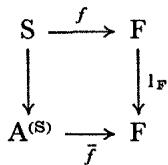
\includegraphics[keepaspectratio]{images/part003_a94682a2.jpg}}

（其中左边的竖直箭头是典范映射 \(s \mapsto e_s\) ）。

设 \(\bar{f}:\mathbf{A}^{(\mathrm{S})}\to\mathbf{F}\) 是唯一的 A-模同态，使得 \(\bar{f}(e_{s})=\bar{f}(s)\) （II，§ 1，第 11 号，命题 17 的推论 3）；只需验证 \(\bar{f}\) 是代数同态，而为此只需证明 \(\bar{f}(e_{s}e_{t})=\bar{f}(e_{s})\bar{f}(e_{t})\) ，它由定义与假设 \(f(st)=f(s)f(t)\) 直接得出。

命题 6 表达了如下事实：由 \(\mathbf{A}^{(\mathbb{S})}\) 与典范映射 \(s\mapsto e_s\) 组成的有序对是泛映射问题（《集合论》，IV，§ 3，第 1 号）的一个解，其中 \(\Sigma\) 是 A-代数结构这一种类，而 \(\alpha\) 映射是把 S 映入一个仅带其乘法律的 A-代数的同态。

推论。设 S, S' 为两个广群， \(g:S\to S'\) 为一个同态。则存在且仅存在一个 A-代数同态 \(u:A^{(S)}\to A^{(S')}\) 使图表交换

\pandocbounded{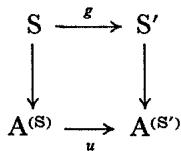
\includegraphics[keepaspectratio]{images/part003_71823134.jpg}}

（其中竖直箭头是典范映射）。

只需把命题 6 应用于取 \(f\) 为复合映射 \(\mathbf{S} \xrightarrow{g} \mathbf{S}' \to \mathbf{A}^{(\mathbf{S}')}\) 的情形。

特别地，若 T 是广群 S（I，§ 1，第 4 号）的稳定子集，则形如 \(\sum_{s\in\mathbf{T}}\alpha_s e_s\) 的元素（属于 \(\mathbf{A}^{(\mathbf{S})}\) ）所成的集合是 \(\mathbf{A}^{(\mathbf{S})}\) 的一个子代数，它典范同构于代数 \(\mathbf{A}^{(\mathbf{T})}\) ，且有时与后者等同。

例。设 V 是一个 A-模，S 是一个在 V 上从左边作用的幺半群；这就是说（I，§ 5，第 1 号），给定了一个映射 \((s, x) \mapsto s.x\) （由 S 到 V），使得 \(s.(x + y) = s.x + s.y\) , \(s.(\alpha x) = \alpha(s.x)\) 与 \(s.(t.x) = (st).x\) 对 \(s, t\) （在 S 中）、 \(x, y\) （在 V 中）与 \(\alpha \in \mathbf{A}\) 成立，且（把 \(e\) 记作 S 的单位元）对 \(x \in V\) 有 e.x = x。写 \(f(s)(x) = s.x\) ，则 f 是 S 到代数 \(\operatorname{End}_{\mathbf{A}}(\mathbf{V})\) （仅带其乘法律）中的一个同态，它把单位元 e 映到单位元 \(1_{V}\) 。应用命题 6，得到一个 A-代数同态 \(\bar{f}: \mathbf{A}^{(\mathbf{S})} \to \operatorname{End}_{\mathbf{A}}(\mathbf{V})\) ，它给出 V 的底群在 \(\mathbf{A}^{(\mathbf{S})}\) 上的一个左模结构。

这使我们能把带算子的交换群的研究归结为模的研究。因为设 M 是一个带算子的交换群，其运算以加法书写，所有外部律以乘法书写。设 \(\Omega\) 为 M 上各个外部律的算子定义域的和集（《集合论》，II，§ 4，第 8 号），其中每个定义域都被典范地等同于 \(\Omega\) 的一个子集。设 \(\mathrm{Mo}(\Omega)\) 为在 \(\Omega\) 上构造的自由幺半群（I，§ 7，第 2 号）；一个作用律

\[
(s, x) \mapsto s. x
\]

在 M 上定义，以 \(\mathrm{Mo}(\Omega)\) 为算子域，通过对 \(\mathrm{Mo}(\Omega)\) 中字 s 的长度作归纳来定义；若 s 的长度为 0，则它是空字 e，我们对所有 \(x \in M\) 写 e.x = x。若 x 的长度为 \(n \geqslant 1\) ，则它可以唯一地写成 s = tu，其中 u 的长度为 n - 1，t 的长度为 1，因此 \(t \in \Omega\) ；随后我们写 s.x = t.(u.x)。对任意两个字 s 与 \(s'\) （在 \(\mathrm{Mo}(\Omega)\) 中），关系 \(s.(s'.x) = (ss').x\) 通过对 s 的长度作归纳来验证。

然后应用上述方法，就在 M 上得到一个左 \(\mathbf{Z}^{(\mathrm{Mo}(\Omega))}\) -模结构，并且不难验证，带算子群论中的通常概念（稳定子群、同态）对带算子的交换群与这样关联于它们的模来说是相同的。

\subsection{自由代数}

定义 2. 设 I 是一个集合；令 M(I)（相应地 Mo(I)，相应地 N \(^{(I)}\) ）表示由 I 导出的自由广群（相应地自由幺半群，相应地自由交换幺半群）。M(I)（相应地 Mo(I)，相应地 N \(^{(I)}\) ）在 A 上的代数称为集合 I 在环 A 上的自由代数（相应地自由结合代数，相应地自由交换结合代数（或作为语言上的滥用，称为自由交换代数））。

我们把 I 在 A 上的自由代数（相应地自由结合代数，相应地自由交换代数）记作 \(\operatorname{Lib}_{\mathbf{A}}(\mathbf{I})\) （相应地 \(\operatorname{Libas}_{\mathbf{A}}(\mathbf{I})\) ，相应地 \(\operatorname{Libasc}_{\mathbf{A}}(\mathbf{I})\) ）。把 I 到 \(\operatorname{M}(\mathbf{I})\) （相应地 \(\operatorname{Mo}(\mathbf{I})\) ，相应地 \(\mathbf{N}^{(\mathbf{I})}\) ）中的典范映射与 \(\operatorname{M}(\mathbf{I})\) （相应地 \(\operatorname{Mo}(\mathbf{I})\) ，相应地 \(\mathbf{N}^{(\mathbf{I})}\) ）到 \(\operatorname{Lib}_{\mathbf{A}}(\mathbf{I})\) （相应地 \(\operatorname{Libas}_{\mathbf{A}}(\mathbf{I})\) ，相应地 \(\operatorname{Libasc}_{\mathbf{A}}(\mathbf{I})\) ）中的典范映射复合，就得到 I 到 \(\operatorname{Lib}_{\mathbf{A}}(\mathbf{I})\) （相应地 \(\operatorname{Libas}_{\mathbf{A}}(\mathbf{I})\) ，相应地 \(\operatorname{Libasc}_{\mathbf{A}}(\mathbf{I})\) ）中的一个典范映射，当 \(A \neq \{0\}\) 时它是单射。我们把元素 \(i \in I\) 在此典范映射下的像记作 \(X_{i}\) ，并称 \(X_{i}\) 为 \(\operatorname{Lib}_{\mathbf{A}}(\mathbf{I})\) （相应地 \(\operatorname{Libas}_{\mathbf{A}}(\mathbf{I})\) ，相应地 \(\operatorname{Libasc}_{\mathbf{A}}(\mathbf{I})\) ）的指标为 i 的未定元。

由于 \(\mathbf{Mo}(\mathbf{I})\) 与 \(\mathbf{N}^{(\mathrm{I})}\) 各有一个单位元， \(\operatorname{Libas}_{\mathbf{A}}(\mathbf{I})\) 与 \(\operatorname{Libasc}_{\mathbf{A}}(\mathbf{I})\)

是含单位元的结合代数，且进一步 \(\operatorname{Libasc}_{\mathbf{A}}(\mathbf{I})\) 是交换的。若 e 是 \(\operatorname{Libas}_{\mathbf{A}}(\mathbf{I})\) （相应地 \(\operatorname{Libasc}_{\mathbf{A}}(\mathbf{I})\) ）的单位元，则映射 \(\alpha \mapsto \alpha e\) 是 A 到 \(\operatorname{Libas}_{\mathbf{A}}(\mathbf{I})\) （相应地 \(\operatorname{Libasc}_{\mathbf{A}}(\mathbf{I})\) ）的中心的一个子环上的同构，该子环与 A 等同（第 1 号）。

命题 7. 设 I 是一个集合，F 是 A 上的一个代数（相应地，含单位元结合代数，相应地，含单位元交换结合代数）。对每个映射 \(f:\mathbf{I}\to\mathbf{F}\) ，存在且仅存在一个同态（相应地，保单位同态） \(\bar{f}\) ，它由 \(\operatorname{Lib}_{\mathbf{A}}(\mathbf{I})\) （相应地 \(\operatorname{Libas}_{\mathbf{A}}(\mathbf{I})\) ，相应地 \(\operatorname{Libasc}_{\mathbf{A}}(\mathbf{I})\) ）到 F 中，使得 \(\bar{f}(\mathbf{X}_{i})=f(i)\) 对所有 \(i\in\mathbf{I}\) 成立。

设 \(F_{m}\) 是通过赋予集合 F 其乘法合成律而得到的广群（相应地，幺半群）。存在且仅存在一个同态（相应地，保单位同态）g，由 M(I)（相应地，Mo(I)，相应地，N \(^{(I)}\) ）到 \(F_{m}\) 中，使得 \(g(i) = f(i)\) 对所有 \(i \in I\) 成立（I，§ 7，第 1、2 与 7 号）；命题 7 随后由第 6 号命题 6 得出。

注记。(1) 我们稍后将定义 \(\operatorname{Libas}_{\mathbf{A}}(\mathbf{I})\) 到自由模 \(\mathbf{A}^{(I)}\) 的张量代数上的一个同构（ \(\S 5\) ，第 5 号），以及 \(\operatorname{Libasc}_{\mathbf{A}}(\mathbf{I})\) 到 \(\mathbf{A}^{(I)}\) 的对称代数上的一个同构（ \(\S 6\) ，第 6 号）。

\begin{enumerate}
\def\labelenumi{(\arabic{enumi})}
\setcounter{enumi}{1}
\item
  设 \(\rho\) 是 A 到交换环 B 中的保单位同态。如已见（§ 2，第 6 号），一个同构 \(\sigma\) 由 \(\rho\) 导出，它把 \(\operatorname{Lib}_{\mathbf{B}}(\mathbf{I})\) （相应地 \(\operatorname{Libas}_{\mathbf{B}}(\mathbf{I})\) ，相应地 \(\operatorname{Libasc}_{\mathbf{B}}(\mathbf{I})\) ）映到代数 \((\operatorname{Lib}_{\mathbf{A}}(\mathbf{I}))_{(\mathbf{B})}\) （相应地 \((\operatorname{Libas}_{\mathbf{A}}(\mathbf{I}))_{(\mathbf{B})}\) ，相应地 \((\operatorname{Libasc}_{\mathbf{A}}(\mathbf{I}))_{(\mathbf{B})}\) ）上，该代数是把标量借助 \(\rho\) 扩张到 B 而得到的；若 \(\mathbf{X}_i^{\mathbf{A}}\) , \(\mathbf{X}_i^{\mathbf{B}}\) 是分别对应于 A 与 B 的指标为 \(i\) 的未定元，则 \(\sigma(\mathbf{X}_i^{\mathbf{B}}) = \mathbf{X}_i^{\mathbf{A}} \otimes 1\) 。
\item
  设 \(J\) 是 \(I\) 的一个子集；我们知道 \(M(J)\) 被等同于广群 \(M(I)\) 的一个稳定子集，因此（第 6 号） \(\operatorname{Lib}_{A}(J)\) 典范地等同于 \(\operatorname{Lib}_{A}(I)\) 的一个子代数，它由诸 \(X_i\) ——满足 \(i \in J\) ——生成；我们说，只有指标属于 \(J\) 的未定元出现在 \(\operatorname{Lib}_{A}(J)\) 的一个元素中。第 6 号中给出的广群代数的定义表明， \(\operatorname{Lib}_{A}(I)\) 是子代数 \(\operatorname{Lib}_{A}(J)\) 的有向族的并，其中 \(J\) 遍历 \(I\) 的有限子集的集合。对 \(\operatorname{Libas}_{A}(I)\) 与 \(\operatorname{Libasc}_{A}(I)\) 有类似的结果。
\item
  对元素 \(s\) —— \(\mathbf{M}(\mathbf{I})\) （相应地 \(\mathbf{Mo}(\mathbf{I})\) ，相应地 \(\mathbf{N}^{(1)}\) ）的——关联它的长度 \(l(s)\) ，这是一个 \(\geqslant 1\) （相应地 \(\geqslant 0\) ）的整数，使得 \(l(ss') = l(s) + l(s')\) （I，§ 7，第 1、2 与 7 号）。若 \(e_s\) 是 \(\operatorname{Lib}_{\mathbf{A}}(\mathbf{I})\) （相应地 \(\operatorname{Libas}_{\mathbf{A}}(\mathbf{I})\) ，相应地 \(\operatorname{Libasc}_{\mathbf{A}}(\mathbf{I})\) ）中对应于 \(s\) 的元素，则元素 \(x = \sum_{s} \alpha_s e_s \neq 0\) （属于 \(\operatorname{Lib}_{\mathbf{A}}(\mathbf{I})\) （相应地 \(\operatorname{Libas}_{\mathbf{A}}(\mathbf{A})\) ，相应地 \(\operatorname{Libasc}_{\mathbf{A}}(\mathbf{I})\) ））的总次数（或简称次数）是诸数 \(l(s)\) 中的最大者，其中 \(s\) 遍历（依假设非空的）满足 \(\alpha_s \neq 0\) 的元素集合。例如，若 \(i, j, k\) 是 \(\mathbf{I}\) 的三个不同元素，则元素 \((\mathrm{X}_t(\mathrm{X}_j\mathrm{X}_k))\mathrm{X}_t - (\mathrm{X}_t\mathrm{X}_j)(\mathrm{X}_k\mathrm{X}_l)\) 是一个 \(\neq 0\) 的、总次数为 4 的元素（在 \(\operatorname{Lib}_{\mathbf{A}}(\mathbf{I})\) 中）。
\end{enumerate}

\subsection{用生成元和关系定义代数}

设 \(\mathbf{F}\) 是 \(\mathbf{A}\) 上的一个代数， \((x_{i})_{i\in I}\) 是 \(\mathbf{F}\) 的元素的一个族。根据第 7 号命题 7，存在唯一的同态 \(f\colon \operatorname{Lib}_{\mathbf{A}}(\mathbf{I})\to \mathbf{F}\) ，使得 \(f(\mathbf{X}_i) = x_i\) 对所有 \(i\in I\) 成立。要使 \(f\) 为满射，必要且充分的条件是 \((x_{i})_{i\in I}\) 是 \(\mathbf{F}\) 的一个生成系。

若 \(\mathbf{U} \in \operatorname{Lib}_{\mathbf{A}}(\mathbf{I})\) ，则 \(f(\mathbf{U})\) 称为 \(\mathbf{F}\) 的、由 \(\mathbf{U}\) 通过把元素 \(x_{i}\) 代入未定元 \(\mathbf{X}_{i}\) 而得到的元素，也称为 \(\mathbf{U}\) 当未定元取值 \(x_{i}\) （就未定元 \(\mathbf{X}_{i}\) 而言）时的值；它通常记作 \(\mathbf{U}((x_{i})_{i \in I})\) ；特别地， \(\mathbf{U}((\mathbf{X}_{i})_{i \in I}) = \mathbf{U}\) 。若 \(\lambda\) 是 \(\mathbf{F}\) 到一个代数 \(\mathbf{F}'\) （ \(\mathbf{A}\) 上的）中的同态，则

\[
\lambda (\mathrm{U} ((x _ {i}) _ {i \in \mathrm{I}})) = \mathrm{U} ((\lambda (x _ {i})) _ {i \in \mathrm{I}}).
\]

特别考虑以下情形： \(\mathrm{F} = \operatorname{Lib}_{\mathbf{A}}(\mathbf{J})\) ，其中 J 是另一个集合；对元素的每一个族 \((\mathrm{H}_{i})_{i \in I}\) （属于 \(\operatorname{Lib}_{\mathbf{A}}(\mathbf{J})\) ）以及每个族 \((y_{j}')_{j \in J}\) （属于 A-代数 \(F'\) ），

\[
\mathrm{U} ((\mathrm{H} _ {i}) _ {i \in I})) ((y _ {j} ^ {\prime}) _ {j \in J}) = \mathrm{U} ((\mathrm{H} _ {i} ((y _ {j} ^ {\prime}) _ {j \in J})) _ {i \in I}).\tag{37}
\]

在上述记号中， \(\operatorname{Lib}_{\mathbf{A}}(\mathbf{I})\) 的每个使得 \(\mathrm{U}((x_{i})_{i\in\mathbf{I}})=0\) （亦即满足 \(f(\mathrm{U})=0\) ）的元素 U，称为族 \((x_{i})_{i\in\mathbf{I}}\) 在 F 中的关系子。由这些元素组成的双边理想 \(\operatorname{Ker}(f)\) 称为 \((x_{i})\) 的关系子理想。

设 \((\mathbf{R}_j)_{j\in J}\) 是 \(\operatorname{Lib}_{\mathbf{A}}(\mathbf{I})\) 的元素的一个族。 \(((x_i)_{i\in I}, (\mathbf{R}_j)_{j\in J})\) 称为代数 \(F\) 的一个表出，如果 \((x_i)_{i\in I}\) 是 \(F\) 的生成系，且 \(\operatorname{Lib}_{\mathbf{A}}(\mathbf{I})\) 的由诸 \(\mathbf{R}_j\) 生成的双边理想等于族 \((x_i)_{i\in I}\) 的关系子理想； \(x_i\) 称为生成元，而 \(\mathbf{R}_j\) 称为该表出的关系子。

现在考虑任意的集合 I 与元素的一个族 \((\mathbf{R}_j)_{j\in J}\) （属于 \(\operatorname{Lib}_{\mathbf{A}}(\mathbf{I})\) ）。 \(\operatorname{Lib}_{\mathbf{A}}(\mathbf{I})\) 关于由族 \((\mathbf{R}_j)\) 生成的双边理想的商代数 E，称为由生成系 I 经关系子族 \((\mathbf{R}_j)_{j\in J}\) 约束而定义的泛代数。显然，若 \(\overline{\mathbf{X}}_i\) 表示 \(\mathbf{X}_i\) 在 E 中的像，

\[
\left(\left(\overline {{\mathbf {X}}} _ {i}\right) _ {i \in I}, \left(\mathbf {R} _ {j}\right) _ {j \in J}\right)
\]

是 E 的一个表出。此外，若 \((x_{i})_{i\in I}\) 是一个代数 F 的元素族，且 \(\mathbf{R}_j((x_i)_{i\in I}) = 0\) 对所有 \(j\in J\) 成立，则存在唯一的同态 \(g:\mathbf{E}\to \mathbf{F}\) ，使得 \(g(\overline{\mathbf{X}}_i) = x_i\) 对所有 \(i\in I\) 成立；要使 \(((x_i)_{i\in I},(\mathbf{R}_j)_{j\in J})\) 是 F 的一个表出，必要且充分的条件是 \(g\) 为双射。

这些评注为下面的语言滥用提供了正当性：不说“ \(((x_i)_{i \in I}, (R_j)_{j \in J})\) 是 F 的一个表出”，也说“F 是由生成元 \(x_i\) 在关系 \(R_j((x_i)_{i \in I}) = 0\) 约束下生成的代数”。当 \(R_j\) 形如 \(P_j - Q_j\) 时，也说“F 是由 \(x_i\) 在关系 \(P_j((x_i)) = Q_j((x_i))\) 约束下生成的代数”。

设 H 是一个集合；我们将说 \(\operatorname{Lib}_{\mathbf{A}}(\mathbf{H})\) 的元素 S 是 A-代数 F 的一个泛关系子，如果 \(\mathrm{S}((x_{h})_{h\in\mathbb{H}})=0\) 对以 H 为指标集的 F 的元素的每个族 \((x_{h})_{h\in\mathbb{H}}\) 成立。

例子。(1) 取 \(\mathbf{H} = \{1,2,3\}\) ；承认

\[
(\mathrm{X} _ {1} \mathrm{X} _ {2}) \mathrm{X} _ {3} - \mathrm{X} _ {1} (\mathrm{X} _ {2} \mathrm{X} _ {3})
\]

作为泛关系子的代数是结合代数。承认 \(X_{1}X_{2}-X_{2}X_{1}\) 作为泛关系子的代数是交换代数。承认泛关系子 \(X_{1}X_{1}\) 与

\[
(\mathrm{X} _ {1} \mathrm{X} _ {2}) \mathrm{X} _ {3} + (\mathrm{X} _ {2} \mathrm{X} _ {3}) \mathrm{X} _ {1} + (\mathrm{X} _ {3} \mathrm{X} _ {1}) \mathrm{X} _ {2}
\]

作为泛关系子的代数是李代数。

设 I 是一个集合；给定元素的一个族 \((\mathrm{S}_{k})_{k\in\mathbb{K}}\) （属于 \(\operatorname{Lib}_{\mathbf{A}}(\mathbf{H})\) ），考虑 \(\operatorname{Lib}_{\mathbf{A}}(\mathbf{I})\) 中形如 \(\mathrm{S}_{k}((\mathrm{U}_{h}))_{h\in\mathbb{H}}\) 的元素组成的集合 T，其中 k 遍历 K，且对每个 \(k,\left(\mathrm{U}_{h}\right)_{h\in\mathbb{H}}\) 遍历 \(\operatorname{Lib}_{\mathbf{A}}(\mathbf{I})\) 的元素的以 H 为指标集的族的集合；再考虑一个以 T 为元素集的族 \((\mathrm{R}_{j})_{j\in\mathbb{J}}\) 。然后令 F 为由生成系 I 经关系子族 \((\mathrm{R}_{j})_{j\in\mathbb{J}}\) 约束而定义的泛代数，并设 \(u:\operatorname{Lib}_{\mathbf{A}}(\mathbf{I})\to\mathbf{F}\) 为典范同态，于是 \(\operatorname{Ker}(u)\) 由形如 \(\mathrm{S}_{k}((\mathrm{U}_{h})_{h\in\mathbb{H}})\) 的元素生成，其中 \(k\in K\) 且 \((\mathrm{U}_{h})_{h\in\mathbb{H}}\) 是 \(\operatorname{Lib}_{\mathbf{A}}(\mathbf{I})\) 的元素的族；显然每个 \(S_{k}\) \((k\in\mathbb{K})\) 都是 F 的一个泛关系子。现在设 \(F'\) 是承认一个生成系 \((x_{i})_{i\in\mathbb{I}}\) 的代数，对它每个 \(S_{k}\) 都是泛关系子，并设 \(u':\operatorname{Lib}_{\mathbf{A}}(\mathbf{I})\to\mathbf{F}'\) 是使得 \(u'(\mathrm{X}_{i})=x_{i}\) （对所有 \(i\in I\) ）成立的同态；显然 \(\operatorname{Ker}(u)\subset\operatorname{Ker}(u')\) ，因此 \(u'\) 可唯一地写成 \(u'=h\circ u\) 的形式，其中 \(h:F\to F'\) 是一个使 \(h(\overline{\mathrm{X}}_{i})=x_{i}\) 对所有 \(i\in I\) 成立的同态。因此，F 称为由生成系 I 定义的、对应于泛关系子族 \((\mathrm{S}_{k})_{k\in\mathbb{K}}\) 的泛代数。作为语言上的滥用，F 有时也称为由 I 生成且满足恒等式 \(\mathrm{S}_{k}((u_{h}))=0\) （对 F 的元素的每个族 \((u_{h})_{h\in\mathbb{H}}\) ）的泛代数。

例 2. 设 \(\mathbf{L}'\) 为由 \(\mathbf{I}\) 生成且满足恒等式 \((uv)w - u(vw) = 0\) （对 \(\mathbf{L}'\) 的元素的每个三元族）的泛代数，并设 \(\mathbf{L}''\) 为由 \(\mathbf{L}'\) 添加单位元而得到的代数；则存在唯一的保单位同构 \(g\) ，它由 \(\mathbf{L}''\) 到 \(\operatorname{Libas}_{\mathbf{A}}(\mathbf{I})\) 上，使得 \(g(\overline{\mathbf{X}}_i) = \mathbf{X}_i\) 对所有 \(i \in \mathbf{I}\) 成立。因为显然 \(\mathbf{L}''\) 是结合的，且同态 \(g\) 的存在性由 \(\mathbf{L}'\) 的定义及其前面的评注得出；但于是显然 \(\mathbf{L}''\) 满足刻画 \(\operatorname{Libas}_{\mathbf{A}}(\mathbf{I})\)

的泛性质（第 7 号，命题 7），由此得出结论。与上述类似的考虑可应用于结合代数（相应地，交换结合代数），同时考虑到以下评注。当上下文充分表明所考虑的代数是含单位元代数时，作为语言上的滥用，一个族 \((x_{i})_{i\in I}\) （它是代数 \(F\) 的元素的族），若由诸 \(x_{i}\) ( \(i\in I\) ) 与单位元生成的子代数等于 \(F\) ，则常称为 \(F\) 的一个生成系。然后设 \(F\) 是 \(A\) 上的一个含单位元结合代数， \((x_{i})_{i\in I}\) 是 \(F\) 的元素的一个族；根据第 7 号命题 7，存在唯一的保单位同态 \(f:\mathrm{Libas}_{\mathbf{A}}(\mathbf{I})\to F\) ，使得 \(f(\mathbf{X}_i) = x_i\) 对所有 \(i\in I\) 成立；若 \(\mathbf{U}\in \mathrm{Libas}_{\mathbf{A}}(\mathbf{I}), f(\mathbf{U})\) 也称为 \(F\) 的、由 \(\mathbf{U}\) 通过把元素 \(x_{i}\) 代入未定元 \(\mathbf{X}_i\) 而得到的元素，并且也记作 \(\mathrm{U}((x_{i})_{i\in I})\) 。于是，关系子、表出与泛关系子的概念可立即搬到结合代数上；只需把 \(\mathrm{Lib}_{\mathbf{A}}(\mathbf{I})\) 处处替换为 \(\mathrm{Libas}_{\mathbf{A}}(\mathbf{I})\) 即可。由生成系 \(I\) 经关系子族 \((\mathbb{R}_j)_{j\in J}\) 约束而定义的泛含单位元结合代数是 \(\mathrm{Libas}_{\mathbf{A}}(\mathbf{I})\) 关于由族 \((\mathbb{R}_j)\) 生成的双边理想的商代数。由生成系 \(I\) 生成的、对应于一族泛关系子的泛含单位元结合代数类似地定义。我们把关于交换结合代数的类似定义的陈述留给读者，只需以 \(\mathrm{Libasc}_{\mathbf{A}}(\mathbf{I})\) 替换 \(\mathrm{Libas}_{\mathbf{A}}(\mathbf{I})\) 即可。

例 3. 设 L' 是由 I 生成且满足恒等式 uv - vu = 0（对 L' 的元素的每个二元族）的泛含单位元结合代数。如例 2 中那样可以看出，L' 典范同构于 \(\text{Libasc}_{\mathbf{A}}(\mathbf{I})\) 。

\subsection{多项式代数}

设 B 是一个含单位元的交换结合 A-代数， \((x_{i})_{i\in I}\) 是 B 的一族元素；由诸 \(x_{i}\) ( \(i\in I\) ) 与单位元生成的 B 的子代数记为 \(\mathrm{A}[(x_{i})_{i\in I}]_{\mathrm{B}}\) ，或在不会引起混淆时简记为 \(\mathrm{A}[(x_{i})_{i\in I}]\) 。对每个集合 I，代数 \(\operatorname{Libasc}_{\mathbf{A}}(\mathbf{I})\) 因此等于 \(\mathrm{A}[(\mathbf{X}_{i})_{i\in I}]\) （也记作 \(\mathrm{A}[\mathbf{X}_{i}]_{i\in I}\) )；后一种记号的优点在于指明了用来表示未定元的记号，我们在本专著的其余部分通常采用它。 \(\mathrm{A}[(\mathbf{X}_{i})_{i\in I}]\) 的元素称为未定元 \(X_{i}\) ( \(i\in I\) ) 的、以 A 中元素为系数的多项式；按约定，当说“设 \(\mathrm{A}[(\mathbf{X}_{i})_{i\in I}]\) 为多项式代数”时，总把 \(X_{i}\) 理解为未定元。对 I 的每个子集 J，使用上述记号相当于把 \(\operatorname{Libasc}_{\mathbf{A}}(\mathbf{J})\) 与 \(\operatorname{Libasc}_{\mathbf{A}}(\mathbf{I})\) 的由诸 \(X_{i}\) （ \(i\in J\) ）与单位元生成的代数（参见第 7 号，注记 (3)）等同起来。对于 \(I=\{1,2,\ldots,n\}\) ，我们记 \(\mathrm{A}[\mathbf{X}_{1},\mathbf{X}_{2},\ldots,\mathbf{X}_{n}]\) 以代替 \(\mathrm{A}[(\mathbf{X}_{i})_{i\in I}]\) 。

若 I 与 I' 是两个等势的集合，则代数 \(\operatorname{Libasc}_{\mathbf{A}}(\mathbf{I})\) 与 \(\operatorname{Libasc}_{\mathbf{A}}(\mathbf{I}')\) 同构。 A{[}X{]} 常用来表示对应于一个只含单个元素的未指明指标集的多项式代数，其中 X 表示唯一的未定元；类似地， A{[}X, Y{]} 、 A{[}X, Y, Z{]} 、 \ldots{} 用来表示对应于具有

2, 3, \ldots{} 个元素。注意，根据上述约定，例如 A{[}X{]} 和 A{[}Y{]} 是 A{[}X, Y, Z{]} 的（不同的）子代数，只要 A ≠ \{0\}。

这些元素

\[
\mathrm{X} ^ {\nu} = \prod_ {i \in I} \mathrm{X} _ {i} ^ {\nu (i)},
\]

其中 v 遍历 \(\mathbf{N}^{(1)}\) ，它们构成多项式代数 \(\mathrm{A}[(\mathrm{X}_{i})_{i\in\mathbb{I}}]\) 的一组基。这些元素称为未定元 \(X_{i}\) 中的单项式，而数 \(|v|=\sum_{i\in\mathbb{I}}v(i)\) 称为单项式 \(X^{v}\) 的次数（或总次数）。唯一的 0 次单项式是 \(\mathrm{A}[(\mathrm{X}_{i})_{i\in\mathbb{I}}]\) 的单位元；它常与 A 的单位元 1 等同。 \(\mathrm{A}[(\mathrm{X}_{i})_{i\in\mathbb{I}}]\) 的每个多项式 u 都可以唯一地写成

\[
u = \sum_ {v \in \mathbf {N} ^ {(I)}} \alpha_ {v} X ^ {v}
\]

其中 \(\alpha_{\nu} \in \mathbf{A}\) ；诸元素 \(\alpha_{\nu}\) ——除有限个指标 \(\nu \in \mathbf{N}^{(1)}\) 外均为零——称为 \(u\) 的系数；诸元素 \(\alpha_{\nu} \mathrm{X}^{\nu}\) 称为 \(u\) 的项（元素 \(\alpha_{\nu} \mathrm{X}^{\nu}\) 常称为“ \(\mathrm{X}^{\nu''}\) 中的项”）；特别地，项 \(\alpha_{0} \mathrm{X}^{0}\) （与 \(\alpha_{0} \in \mathbf{A}\) 等同）称为 \(u\) 的常数项。若 \(J\) 是 \(I\) 的子集，则 \(u\) 属于 \(\mathrm{A}[(\mathrm{X}_{i})_{i \in J}]\) 当且仅当 \(\alpha_{\nu} = 0\) 对所有 \(\nu \notin \mathbf{N}^{(J)}\) 成立。由此可得 \(\mathrm{A}[(\mathrm{X}_{i})_{i \in I}]\) 是诸子代数 \(\mathrm{A}[(\mathrm{X}_{i})_{i \in J}]\) 的并，其中 \(J\) 遍历 \(I\) 的有限子集组成的集合。若 \(\alpha_{\nu} = 0\) 对所有 \(|\nu| > n\) 成立，则 \(u\) 称为次数 \(\leqslant n\) 的多项式。当 \(\alpha_{\nu} = 0\) 时，（作为语言上的滥用）称 \(u\) 不含 \(\mathrm{X}^{\nu'}\) 中的项；特别地，当 \(\alpha_{0} = 0\) 时， \(u\) 称为无常数项的多项式。

对每个非零多项式 \(u = \sum_{v} \alpha_v X^v\) ， \(u\) 的次数（或总次数）是整数 \(|v|\) 中最大的一个，其中 \(v\) 是满足 \(\alpha_v \neq 0\) 的多重指标。

设 F 为 A 上的一个含单位元结合代数， \((x_{i})_{i\in I}\) 为 F 的一族两两可交换的元素。F 的子代数 \(F'\) ——由诸 \(x_{i}\) 与单位元生成——是交换的（§1，第 7 号），这使我们可以定义把诸 \(x_{i}\) 代入诸 \(X_{i}\) （在多项式 \(u\in\mathrm{A}[(X_{i})_{i\in I}]\) 中；尽管 F 未必交换）： \(u((x_{i})_{i\in I})\) 是 \(F'\) 的、从而是 F 的元素，而 \(h\colon u\to u((x_{i})_{i\in I})\) 是 \(\mathrm{A}[(X_{i})_{i\in I}]\) 到 F 中的一个同态。同态 h 的核的元素称为族 \((x_{i})\) 在 \(\mathrm{A}[(X_{i})_{i\in I}]\) 中的关系子，也称为诸 \(x_{i}\) 之间的（系数在 A 中的）多项式关系子。同态 h 的像是子代数 \(F'\) ，也记作 \(\mathrm{A}[(x_{i})_{i\in I}]\) （即使 F 不交换时亦然）；若 a 是诸 \(x_{i}\) 之间的多项式关系子的理想，则存在 A-模的正合序列

\[
0 \longrightarrow a \longrightarrow A [ (X _ {i}) _ {i \in I} ] \stackrel {h} {\longrightarrow} A [ (x _ {i}) _ {i \in I} ] \longrightarrow 0.
\]

命题 8. 设 \(\mathbf{A}[(\mathbf{X}_i)_{i\in I}]\) 是一个多项式代数， \(J\) 是 \(I\) 的一个子集， \(K\) 是 \(J\) 在 \(I\) 中的补集。记 \(\mathbf{A}' = \mathbf{A}[(\mathbf{X}_j)_{j\in J}]\) ，并用 \(\mathbf{X}_k'\) ( \(k\in K\) ) 表示多项式代数 \(\operatorname{Libasc}_{\mathbf{A}'}(\mathbf{K}) = \mathbf{A}'[(\mathbf{X}_k')_{k \in \mathbb{K}}]\) 中的未定元，则存在唯一的环同构，它由 \(\mathbf{A}'[(\mathbf{X}_k')_{k \in \mathbb{K}}]\) 映到 \(\mathbf{A}[(\mathbf{X}_i)_{i \in I}]\) 上，在 \(\mathbf{A}'\) 上与恒等映射一致，并把 \(\mathbf{X}_k'\) 映为 \(\mathbf{X}_k\) （对所有 \(k \in \mathbb{K}\) ）。

显然 \(\mathbf{A}[(\mathbf{X}_i)_{i\in I}]\) 是一个 \(\mathbf{A}'\) -代数，由诸 \(\mathbf{X}_k\) （对于 \(k\in \mathbf{K}\) ）生成。另一方面，由于诸 \(\mathbf{X}_k\) ( \(k\in \mathbf{K}\) ) 之间的、系数在 \(\mathbf{A}'\) 中的多项式关系子都可以唯一地写成 \(\sum_{\nu}h_{\nu}((\mathbf{X}_j)_{j\in J})\mathbf{X}^{\nu}\) ，其中 \(\nu\) 遍历 \(\mathbf{N}^{(\mathbb{R})}\) 的一个有限子集，且诸 \(h_\nu\) 是 \(\mathbf{A}[(\mathbf{X}_j)_{j\in J}]\) 的元素，故诸 \(h_\nu\) 必是诸 \(\mathbf{X}_j\) 之间的、系数在 \(\mathbf{A}\) 中的多项式关系子，从而全为零，这就证明了该命题。

命题 8 中所述的同构常被用来把 \(\mathbf{A}[(\mathbf{X}_i)_{i\in I}]\) 的元素与系数在 \(\mathbf{A}' = \mathbf{A}[(\mathbf{X}_j)_{j\in J}]\) 中的多项式等同起来。若 \(u\) 是一个 \(\neq 0\) 的元素（属于 \(\mathbf{A}[(\mathbf{X}_i)_{i\in I}]\) ），则它作为 \(\mathbf{A}'[(\mathbf{X}_k)_{k\in K}]\) 的元素而考虑的总次数也称为它关于诸 \(\mathbf{X}_i\) ——指标为 \(i\in K\) ——的次数。

注记。设 I 与 J 是两个集合， \((\mathrm{P}_{j})_{j\in J}\) 是 \(\mathbf{Z}[(\mathrm{X}_{i})_{i\in I}]\) 的元素的一个族；若 Q 是 \(\mathbf{Z}[(\mathrm{X}_{j})_{j\in J}]\) 的一个使得 \(\mathbf{Q}((\mathrm{P}_{j})_{j\in J})=0\) 的元素，则对环 B 中两两可交换元素的每个族 \((b_{i})_{i\in I}\)

\[
\mathrm{Q} ((\mathrm{P} _ {j} ((b _ {i}) _ {i \in \mathrm{I}})) _ {j \in \mathrm{J}}) = 0.
\]

成立的形如 \(\mathbf{Q}((\mathbf{P}_{j})_{j\in\mathbf{J}})=0\) 的关系有时称为多项式恒等式。例如

\[
\left(\mathrm{X} _ {1} + \mathrm{X} _ {2}\right) ^ {2} - \mathrm{X} _ {1} ^ {2} - \mathrm{X} _ {2} ^ {2} - 2 \mathrm{X} _ {1} \mathrm{X} _ {2} = 0
\]

使得

\[
\begin{array}{r l} \mathrm{Q} & = \mathrm{Y} _ {1} ^ {2} - \mathrm{Y} _ {2}, \qquad \mathrm{P} _ {1} = \mathrm{X} _ {1} + \mathrm{X} _ {2}, \qquad \mathrm{P} _ {2} = \mathrm{X} _ {1} ^ {2} + \mathrm{X} _ {2} ^ {2} + 2 \mathrm{X} _ {1} \mathrm{X} _ {2} \\ & \quad \mathrm{X} _ {1} ^ {n} - \mathrm{X} _ {2} ^ {n} - (\mathrm{X} _ {1} - \mathrm{X} _ {2}) (\mathrm{X} _ {1} ^ {n - 1} + \mathrm{X} _ {1} ^ {n - 2} \mathrm{X} _ {2} + \dots + \mathrm{X} _ {2} ^ {n - 1}) = 0 \end{array}
\]

使得

\[
\begin{array}{c} \mathrm{Q} = \mathrm{Y} _ {1} - \mathrm{Y} _ {2} \mathrm{Y} _ {3}, \qquad \mathrm{P} _ {1} = \mathrm{X} _ {1} ^ {n} - \mathrm{X} _ {2} ^ {n}, \qquad \mathrm{P} _ {2} = \mathrm{X} _ {1} - \mathrm{X} _ {2}, \\ \mathrm{P} _ {3} = \mathrm{X} _ {1} ^ {n - 1} + \mathrm{X} _ {1} ^ {n - 2} \mathrm{X} _ {2} + \dots + \mathrm{X} _ {2} ^ {n - 1} \end{array}
\]

是多项式恒等式。

\subsection{幺半群的全代数}

幺半群 S 在 A 上的代数（作为 A-模）是积 \(A^{s}\) 中由具有有限支集的族 \((\alpha_{s})_{s\in\mathbb{S}}\) 组成的子模；这个代数中的乘法由关系式 \((\alpha_{s})(\beta_{s})=(\gamma_{s})\) 定义，其中，对所有 \(s\in S\) ，

\[
\gamma_ {s} = \sum_ {t u = s} \alpha_ {t} \beta_ {u}\tag{38}
\]

（参见第 6 号，公式 (35)）。式 (38) 右端的和是有意义的，因为 \((\alpha_{s})\) 和 \((\beta_{s})\) 都是有限支集的族，从而双重族 \((\alpha_{t}\beta_{u})_{(t,u)\in S\times S}\) 也是有限支集的。但式 (38) 的右端对任意元素 \((\alpha_{s})\) , \(\beta_{s})\) （属于 \(A^{S}\) ）也是有意义的，只要幺半群 \(S\) 满足以下条件：

\begin{enumerate}
\def\labelenumi{(\Alph{enumi})}
\setcounter{enumi}{3}
\tightlist
\item
  对所有 \(s \in \mathbf{S}\) ，只存在有限多个有序对 \((t, u)\) —— \(\mathbf{S} \times \mathbf{S}\) 中的——，使得 \(tu = s\) 。
\end{enumerate}

现在假设 S 满足条件 (D)；此时可以在乘积 A-模 \(A^{s}\) 上由公式 (38) 定义一个乘法。立即可见，这样定义在 \(A^{s}\) 上的乘法是 A-双线性的；它也是结合的，因为对于 \(\alpha\) , \(\beta\) , \(\gamma\) （属于 \(A^{s}\) ），

\[
\sum_ {u v w = t} \alpha_ {u} \beta_ {v} \gamma_ {w} = \sum_ {r w = t} \left(\left(\sum_ {u v = r} \alpha_ {u} \beta_ {v}\right) \gamma_ {w}\right) = \sum_ {u s = t} \left(\alpha_ {u} \left(\sum_ {v w = s} \beta_ {v} \gamma_ {w}\right)\right).
\]

该乘法与 \(A^{s}\) 上的 A-模结构一起，在 \(A^{s}\) 上定义了一个 A 上的含单位元结合代数结构；我们称集合 \(A^{s}\) 连同此结构为幺半群 S 在 A 上的全代数。

立即可见，代数 \(\mathbf{A}^{(\mathbf{S})}\) ——幺半群 \(\mathbf{S}\) 在 \(\mathbf{A}\) 上的——（在需要避免混淆时也称 \(\mathbf{S}\) 的限制代数）是幺半群 \(\mathbf{S}\) 在 \(\mathbf{A}\) 上的全代数的一个子代数（且当 \(\mathbf{S}\) 有限时与后者相同）。作为语言上的滥用，全代数的每个元素 \((\xi_s)_{s \in \mathbf{S}}\) （ \(\mathbf{S}\) 在 \(\mathbf{A}\) 上的）也沿用同样的记号 \(\sum_{s \in \mathbf{S}} \xi_s e_s\) （或甚至 \(\sum_{s \in \mathbf{S}} \xi_s s\) ）—— \(\mathbf{S}\) 的限制代数的元素所用的记号——；当然，这个记号中出现的求和符号不对应任何代数运算，因为它一般是对无穷多个 \(\neq 0\) 的项取的。利用这一记号， \(\mathbf{S}\) 的全代数中的乘法也由第 6 号的公式 (35) 给出。

若 S 是交换的，则它的全代数 \(A^{S}\) 也是交换的。若 T 是 S 的子幺半群，则幺半群的全代数 \(A^{T}\) 典范地等同于 S 的全代数的一个子代数。若 \(\rho: A \to B\) 是环同态，则典范扩张 \(\rho^{S}: A^{S} \to B^{S}\) 是从 S 在 A 上的全代数到 S 在 B 上的全代数中的 A-同态，它扩张了典范同态 \(A^{(S)} \to B^{(S)}\) 。
